\graphicspath{{content/chapters/3_methodology/figures/}}

\chapter{Methodology}
\label{chp:methodology}

This chapter describes the experimental pipeline underlying the empirical analyses presented in this thesis. Figure~\ref{fig:methodology_overview} summarises the six principal stages and their interdependencies.

Section~\ref{sec:image_retrieval} describes Re-LAION-5B image retrieval and embedding computation. Section~\ref{sec:profession_retrieval} details the construction and filtering of profession-conditioned image subsets across 200 occupations. Section~\ref{sec:generation_pipeline} describes the Stable Diffusion v1.5 generation pipeline and validation procedure. Section~\ref{sec:demographic_annotation} presents the gender and Monk Skin Tone annotation pipeline. Section~\ref{sec:transformation_pipeline} describes the transformation-based probing framework, and Section~\ref{sec:debiased_generation} presents the inference-time debiasing pipeline.

\begin{figure}[htbp]
	\centering
	\includegraphics[width=\textwidth]{methodology_overview}
	\caption{Overview of the methodology pipeline.}
	\label{fig:methodology_overview}
\end{figure}


\section{Image Retrieval}
\label{sec:image_retrieval}

This section describes the data acquisition process applied to Re-LAION-2B-en-research-safe, covering shard subsetting, image validity criteria, URL decay, and CLIP embedding computation.

\subsection{Data Acquisition and Subsetting}
\label{subsec:data_acquisition}

Re-LAION-2B-en-research-safe is distributed as 128 shards of approximately 3.62\,GB each. Due to storage and computational constraints, processing was restricted to four randomly selected shards, yielding 65,552,809 URL--caption pairs. Because LAION shards are generated during distributed web crawling without semantic ordering, shard index does not correspond to content category, domain, or temporal structure; random selection therefore supports treating the subset as representative of the broader corpus. Under a binomial sampling model, this scale yields a worst-case 95\% margin of error of approximately $\pm 0.04\%$ for proportion estimates. Nonetheless, unknown crawl-time biases such as domain saturation effects cannot be excluded without access to LAION crawl metadata, and all findings are reported as representative estimates rather than exact population parameters.

\subsection{Image Source Distribution}
\label{subsec:image_source}

Analysis of valid image origins showed that 18.79\% of successfully retrieved images came from five domains: \texttt{cdn.shopify.com} (3,053,782 images), \texttt{i.pinimg.com} (2,585,519), \texttt{i.ebayimg.com} (966,820), \texttt{images-na.ssl-images-amazon.com} (886,054), and \texttt{thumbs.dreamstime.com} (678,516). This concentration indicates strong domain centralisation, with large commercial platforms contributing disproportionately to the retrieved pool. Product imagery and stock photography may therefore be overrepresented relative to content from smaller independent domains.

\subsection{Image Validity Criteria}
\label{subsec:image_validity}

Since Re-LAION-5B distributes URL--caption pairs rather than image binaries, each URL had to be resolved before downloading the image. An image was retained only if it satisfied all of the following conditions: a GET request completed successfully with an HTTP 2xx status code within a 10-second timeout; the response body was successfully decoded and converted to RGB; and embedding computation succeeded. Where embedding computation failed for a batch, recursive binary splitting was applied to isolate and exclude individual corrupted images without falling back to serial processing.

\subsection{Decay Rate}
\label{subsec:decay_rate}

From 65,552,809 attempted URLs, 43,491,938 images were retrieved and validated, yielding a decay rate of:

\[
	\text{Decay Rate} = 1 - \frac{43{,}491{,}938}{65{,}552{,}809} \approx 0.337
\]

This level of link attrition is consistent with prior observations of web-scale dataset degradation \cite{Klein_2014_LinkRot, Schuhmann_2022_Laion5b}. Link decay is not necessarily uniform: if domains or content types become unavailable at different rates, the surviving image pool may be skewed relative to the original dataset, introducing survivorship bias that cannot be quantified post-hoc.

\subsection{Image Preprocessing and Embedding Computation}
\label{subsec:embedding_computation}

All images were preprocessed using the canonical \texttt{openai/clip-vit-large-patch14} pipeline: resizing to 224$\times$224 pixels with aspect-ratio preservation, centre cropping, and CLIP-specific channel normalisation. CLIP image embeddings were extracted using the same model (embedding dimensionality: 768; patch resolution: 14$\times$14) under \texttt{torch.no\_grad()} in evaluation mode with GPU acceleration.

Each embedding vector $\mathbf{e}$ was L2-normalised:

\[
	\mathbf{e}_{\mathrm{norm}} = \frac{\mathbf{e}}{\|\mathbf{e}\|_2}
\]

This enforces unit-length representations and enables cosine similarity retrieval via inner-product equivalence, as described in Section~\ref{subsec:faiss_index}. Results were incrementally flushed to Parquet files with checkpointing for fault tolerance and resumability.

While the original LAION-5B filtering pipeline employed CLIP ViT-B/32, this work uses the higher-capacity ViT-L/14 variant, which offers 768-dimensional embeddings, finer spatial granularity, and stronger semantic alignment in retrieval benchmarks. Since the objective is bias analysis rather than replication of LAION filtering thresholds, using a higher-capacity backbone is methodologically appropriate. The pipeline was executed on an NVIDIA RTX 3060 Ti GPU with 64\,GB of system RAM over approximately two to three months.

Images were accessed exclusively via publicly available URLs furthermore, no authentication mechanisms were bypassed, no image binaries were redistributed, and no attempt was made to identify individuals. Analysis was conducted only at aggregate statistical levels to characterise bias, not to make individual-level demographic predictions or deploy demographic classification systems.

The retrieval process has five primary limitations: only 4 of 128 shards were processed; unknown crawl-time biases cannot be excluded without LAION crawl metadata; 33.7\% of URLs were unavailable; five platforms account for 18.79\% of valid images; and embeddings remain dependent on the CLIP encoder and its pretraining biases.

\section{Profession-Conditioned Image Retrieval}
\label{sec:profession_retrieval}

This section describes how the 43 million retrieved embeddings were used to construct 200 profession-conditioned subsets, covering FAISS indexing, retrieval prompts, filtering, and the statistical justification for the 1,000-image-per-profession design.

\subsection{Profession-Conditioned Subset Construction}
\label{subsec:profession_subset_construction}

Following embedding computation, profession-conditioned imagery was selected as the primary analytical lens because occupational prompts provide an interpretable probe for learned demographic priors, as established in Section~\ref{sec:occupations}. A set of 200 professions was aligned with ISCO-08 categories to ensure systematic coverage across skill levels and domains; the full list is provided in Appendix \ref{app:occupation_list}.

An image is considered valid if it contains exactly one clearly detectable face associated with an identifiable person bounding box and satisfies the spatial and anatomical consistency criteria used in both pipelines. The retrieval-specific filtering procedure is described in Section~\ref{subsec:structural_validation_retrieval}, and the corresponding generation validation procedure is described in Section~\ref{subsec:structural_validation}.


\subsection{FAISS Index Construction}
\label{subsec:faiss_index}

To enable similarity-based retrieval over the 43 million L2-normalised embeddings, a FAISS IndexFlatIP index and position-to-path mapping were constructed per shard. Since embeddings were L2-normalised during extraction, inner product search over IndexFlatIP is equivalent to cosine similarity retrieval. Index construction processed each Parquet file row-group by row-group, with atomic checkpointing for crash recovery. At retrieval time, shard indexes were streamed sequentially, aggregated, and globally re-ranked by similarity score.

\subsection{Prompt Design}
\label{subsec:retrieval_prompt}

The retrieval template used for each profession was:

\[
	\texttt{"A photo of a/an \{profession\}"}
\]

The grammatical article was assigned programmatically based on the profession name. Gender-neutral phrasing was used to avoid reinforcing gender priors during retrieval.

\subsection{Negative Prompt Dominance Filtering}
\label{subsec:negative_filtering}

A negative prompt dominance filter suppressed semantically irrelevant retrievals. For each candidate image, its CLIP embedding was compared against embeddings derived from the following negative prompts: Cartoon, NSFW, Sex, Naked, Clothing, Object, Sign, Logo, Document, Paper, Page, Animal. A candidate was rejected if the maximum cosine similarity to any negative concept satisfied:

\[
	\text{sim}_{\text{neg}} \geq \text{sim}_{\text{pos}} - \delta
\]

where $\text{sim}_{\text{pos}}$ is the cosine similarity to the target profession prompt and $\delta = 0.01$ is a dominance margin. This enforces strict positive dominance: an image is retained only when the target profession prompt exceeds every negative concept by more than the margin.

\subsection{Embedding-Level Deduplication}
\label{subsec:deduplication}

To prevent duplicates within a profession's result set, each candidate embedding was hashed by byte representation and duplicate hashes were discarded before accumulation. Cross-profession deduplication was not enforced as the same image could be relevant to multiple professions.

\subsection{Retrieval Parameters}
\label{subsec:retrieval_params}

For each profession, the top 125,000 candidates were retrieved per shard and aggregated globally. A cosine similarity threshold of 0.15 removed near-random matches while preserving a large candidate pool for structural filtering. Following structural validation, the top 1,000 retrieval prompt aligned images were retained per profession. This two-stage design decouples semantic relevance from structural suitability.

\subsection{Face Detection Model Selection}
\label{subsec:face_detection_selection}

Face detection is a critical gating step in both retrieval and generation pipelines: images without a clearly detectable face are rejected before demographic annotation, as systematic failure on specific face scales or poses would introduce filtering bias. Four candidate models were evaluated on WIDER Face \cite{Yang_2016_WIDERFace}, reporting AP@0.5 overall, AP@0.5 by face size, and COCO-style mAP. Table~\ref{tab:face_det_eval} summarises all results and Figure~\ref{fig:face_det_pr} shows the corresponding precision-recall curves.

MediaPipe \cite{Lugaresi_2019_MediaPipe} achieved only 0.117 AP@0.5 with zero small-face recall, consistent with its design as a conservative single-face detector for mobile inference. RetinaFace \cite{Deng_2020_RetinaFace}, evaluated via the \texttt{batch\_face} library, achieved 0.319 AP@0.5 with near-zero small-face recall; the precision-recall curve reveals systematic detection suppression rather than a precision-recall trade-off, and the library-level deviation from the original implementation limits interpretability. SCRFD \cite{Guo_2021_SCRFD} achieved 0.844 AP@0.5 overall but its small-face AP of 0.614 falls substantially below YOLOv12l-Face. YOLOv12l-Face achieved the highest AP@0.5 (0.905), highest mAP@0.50:0.95 (0.556), and best small-face AP (0.783). Its precision-recall curve sustains near-perfect precision to approximately 0.8 recall, wider than SCRFD, which begins degrading at around 0.6 recall. YOLOv12l-Face was therefore selected as the face detection model for all filtering and annotation pipelines.

\begin{table}[H]
	\centering
	\footnotesize 
	\begin{tabular}{llllll}
		\hline
		\textbf{Model}         & \textbf{AP@0.5} & \textbf{mAP@0.5:0.95} &
		\textbf{Small}         & \textbf{Medium} & \textbf{Large}                                         \\
		\hline
		\textbf{YOLOv12l-Face} & \textbf{0.905}  & \textbf{0.556}        &
		\textbf{0.783}         & \textbf{0.915}  & 0.948                                                  \\
		SCRFD                  & 0.844           & 0.478                 & 0.614 & 0.884 & \textbf{0.954} \\
		RetinaFace$^\dagger$   & 0.319           & 0.176                 & 0.011 & 0.376 & 0.712          \\
		MediaPipe              & 0.117           & 0.040                 & 0.000 & 0.015 & 0.497          \\
		\hline
	\end{tabular}
	\caption{Face detection model evaluation on the WIDER Face validation
		set. AP@0.5 is reported overall and stratified by face size.
		mAP@0.50:0.95 is the COCO-style average across IoU thresholds.
		$^\dagger$ Evaluated using the \texttt{batch\_face} library, which
		uses a different model checkpoint and preprocessing pipeline from
		the original RetinaFace implementation; results reflect this
		deployment configuration rather than the model's published
		capability.}
	\label{tab:face_det_eval}
\end{table}

\begin{figure}[H]
	\centering
	\includegraphics[width=0.48\textwidth]{pr_retinaface.png}
	\includegraphics[width=0.48\textwidth]{pr_scrfd.png}\\[6pt]
	\includegraphics[width=0.48\textwidth]{pr_mediapipe.png}
	\includegraphics[width=0.48\textwidth]{pr_yolov12.png}
	\caption{Precision-recall curves at IoU$=0.5$ on the WIDER Face
		validation set for all four evaluated face detection models.
		RetinaFace and MediaPipe both exhibit a recall ceiling below
		0.35 at near-perfect precision, indicating systematic detection
		suppression. SCRFD maintains high precision to approximately
		0.6 recall before degrading. YOLOv12l-Face achieves the widest
		high-precision operating range, sustaining near-perfect precision
		to approximately 0.8 recall, consistent with its superior AP@0.5
		and small-face detection performance.}
	\label{fig:face_det_pr}
\end{figure}

\subsection{Human-Centric Structural Filtering}
\label{subsec:structural_validation_retrieval}

CLIP-based retrieval does not guarantee clearly identifiable individuals; therefore, a multi-stage structural validation pipeline was applied to enforce human-centric suitability. Images were loaded in batches using TurboJPEG for JPEG inputs, with OpenCV as fallback. Face detection required exactly one detected face with confidence $\geq 0.6$; person detection required at least one detected person with confidence $\geq 0.5$.

Following face detection, MediaPipe FaceMesh was applied to the detected face region. Images for which FaceMesh failed to return landmarks were discarded. For successful FaceMesh detections, landmarks defined a convex hull mask from which a tightly cropped face ROI was extracted with 10-pixel padding. Spatial consistency was then verified by requiring the face centroid to lie within a person bounding box, or IoU between the face and person bounding boxes to be $\geq 0.3$, with a face-to-person area ratio exceeding $0.02$. Images with a valid face and successful FaceMesh segmentation were retained even when person detection was imperfect, avoiding unnecessary rejection where the face was clearly detectable but the person bounding box was slightly misaligned.

\subsection{Filtering Outcomes and Acceptance Rate Distribution}
\label{subsec:filtering_outcomes}

Across all 200 professions, 25,125,679 candidate images were submitted for structural validation, of which 8,420,684 satisfied all criteria, yielding a mean acceptance rate of 33.51\% (median 33.67\%, standard deviation 10.71\%).

Figure~\ref{fig:acceptance_histogram} illustrates the distribution of per-profession acceptance rates. The distribution is approximately unimodal with a visible left tail, consistent with the expectation that CLIP retrieval quality is profession-dependent: occupations associated with clear single-person visual conventions yield more structurally valid results than those whose online representation is dominated by equipment, environments, or group scenes. The 66\% rejection rate confirms that CLIP retrieval alone is insufficient for demographic analysis.

\begin{figure}[H]
	\centering
	\includegraphics[width=\textwidth]{ReLaion-Distribution.png}
	\caption{Distribution of structural acceptance rates across 200 professions
		following CLIP retrieval and YOLO-based structural filtering of Re-LAION-5B
		images. The distribution is approximately unimodal with a mean of 33.51\%
		and median of 33.67\%, with a visible left tail reflecting professions whose
		online visual representation is dominated by non-person content.}
	\label{fig:acceptance_histogram}
\end{figure}

\subsection{Subset Design and Statistical Justification}
\label{subsec:subset_design}

For each of the 200 professions, 1,000 images were retained following structural validation, yielding a balanced profession-conditioned subset of 200,000 images. Under a binomial model for binary feature presence, a per-profession sample of $n = 1{,}000$ yields a worst-case 95\% margin of error of:

\[
	\text{MOE} = z_{0.975} \cdot \sqrt{\frac{p(1-p)}{n}} = 1.96 \cdot
	\sqrt{\frac{0.25}{1000}} \approx \pm 3.1\%
\]

This margin is sufficient to detect meaningful cross-profession differences in spurious feature prevalence. Aggregating across all 200 professions yields a 200,000-image subset, for which binary proportion estimates have a worst-case 95\% margin of error of approximately $\pm 0.22\%$. Equal sampling prevents high-frequency professions from dominating aggregate statistics, but means aggregate prevalence estimates reflect an equal-weighted occupational average rather than the natural profession frequency distribution within Re-LAION-5B.

\section{Image Generation Pipeline}
\label{sec:generation_pipeline}

This section describes the synthetic corpus generated using Stable Diffusion v1.5 with LCM-LoRA acceleration, covering model selection, prompt design, guidance scale rationale, and structural validation.

\subsection{Model Selection}
\label{subsec:gen_model_selection}

A corresponding synthetic image set was required to compare training data with generative model outputs. Model selection was governed by two criteria: traceability to a documented LAION-derived corpus and throughput sufficient to generate 200,000 images within available constraints.

Applying the traceability criterion first, candidate models were restricted to those with a publicly documented training lineage derived from Re-LAION-5B. Three configurations satisfied this requirement: Stable Diffusion v1.5 \cite{StableDiffusion_2022_SD15modelcard}, SD v1.5 with LCM-LoRA \cite{StableDiffusion_2022_SD15modelcard, LCMLoRA_SDv15}, and Stable Diffusion v1.2 \cite{SD12_ModelCard}, all trained exclusively on LAION-Aesthetics v2 5+ \cite{Schuhmann_2022_LaionAesthetics}. Subsequent iterations were excluded: Stable Diffusion 2.0 and 2.1 employed a different text encoder architecture \cite{Cherti_2023_OpenCLIP} introducing confounds; SDXL, Stable Diffusion 3, and later releases were trained on proprietary datasets of undisclosed composition \cite{Podell_2023_SDXL, Esser_2024_SD3}, severing the documentable link to Re-LAION-5B that this analysis requires.\footnote{Additional architectures screened during preliminary evaluation --- SSD-1B \cite{SSD1B_ModelCard}, PixArt-Alpha \cite{PixArtAlpha_ModelCard}, and Segmind Vega \cite{SegmindVega_ModelCard} --- were excluded solely on the basis of training data provenance.}

Among the three qualifying configurations, final selection was based on inference throughput. Per-image inference times are reported in Table~\ref{tab:generative-model-inference-time}. SD v1.5 with LCM-LoRA achieved 1.5 seconds per image, compared to 5.6 seconds for standard SD v1.5 and 9.1 seconds for SD v1.2. At 200,000 images, this corresponds to approximately 83 hours versus 311 hours, making the LCM-accelerated configuration the only feasible option within the available compute window.

\begin{table}[htbp]
	\centering
	\footnotesize
	\begin{tabular}{lcc}
		\toprule
		\textbf{Model} & \textbf{Training Corpus} & \textbf{Time (s/image)} \\
		\midrule
		SD v1.5 LCM-LoRA$^\dagger$~\cite{StableDiffusion_2022_SD15modelcard, LCMLoRA_SDv15}
		               & LAION-Aesthetics v2 5+   & 1.5                     \\
		SD v1.5~\cite{StableDiffusion_2022_SD15modelcard}
		               & LAION-Aesthetics v2 5+   & 5.6                     \\
		SD v1.2~\cite{SD12_ModelCard}
		               & LAION-Aesthetics v2 5+   & 9.1                     \\
		\bottomrule
	\end{tabular}
	\caption{Per-image inference times for LAION-derived model configurations
		at 512$\times$512 resolution. Times are the mean over four generation runs
		on an NVIDIA RTX 3060 Ti. $^\dagger$LCM-LoRA acceleration applied.}
	\label{tab:generative-model-inference-time}
\end{table}

Sample outputs from each configuration are shown in Figure~\ref{fig:model_comparison_samples}. SD v1.5 and SD v1.5 LCM-LoRA both produce consistently full-body, anatomically plausible compositions, with SD v1.5 LCM-LoRA retaining structural reliability at substantially reduced inference cost and only a marginal reduction in fine texture detail. SD v1.2 produces outputs of comparable quality but at 9.1 seconds per image, offering no throughput advantage.

\begin{figure}[htbp]
	\centering
	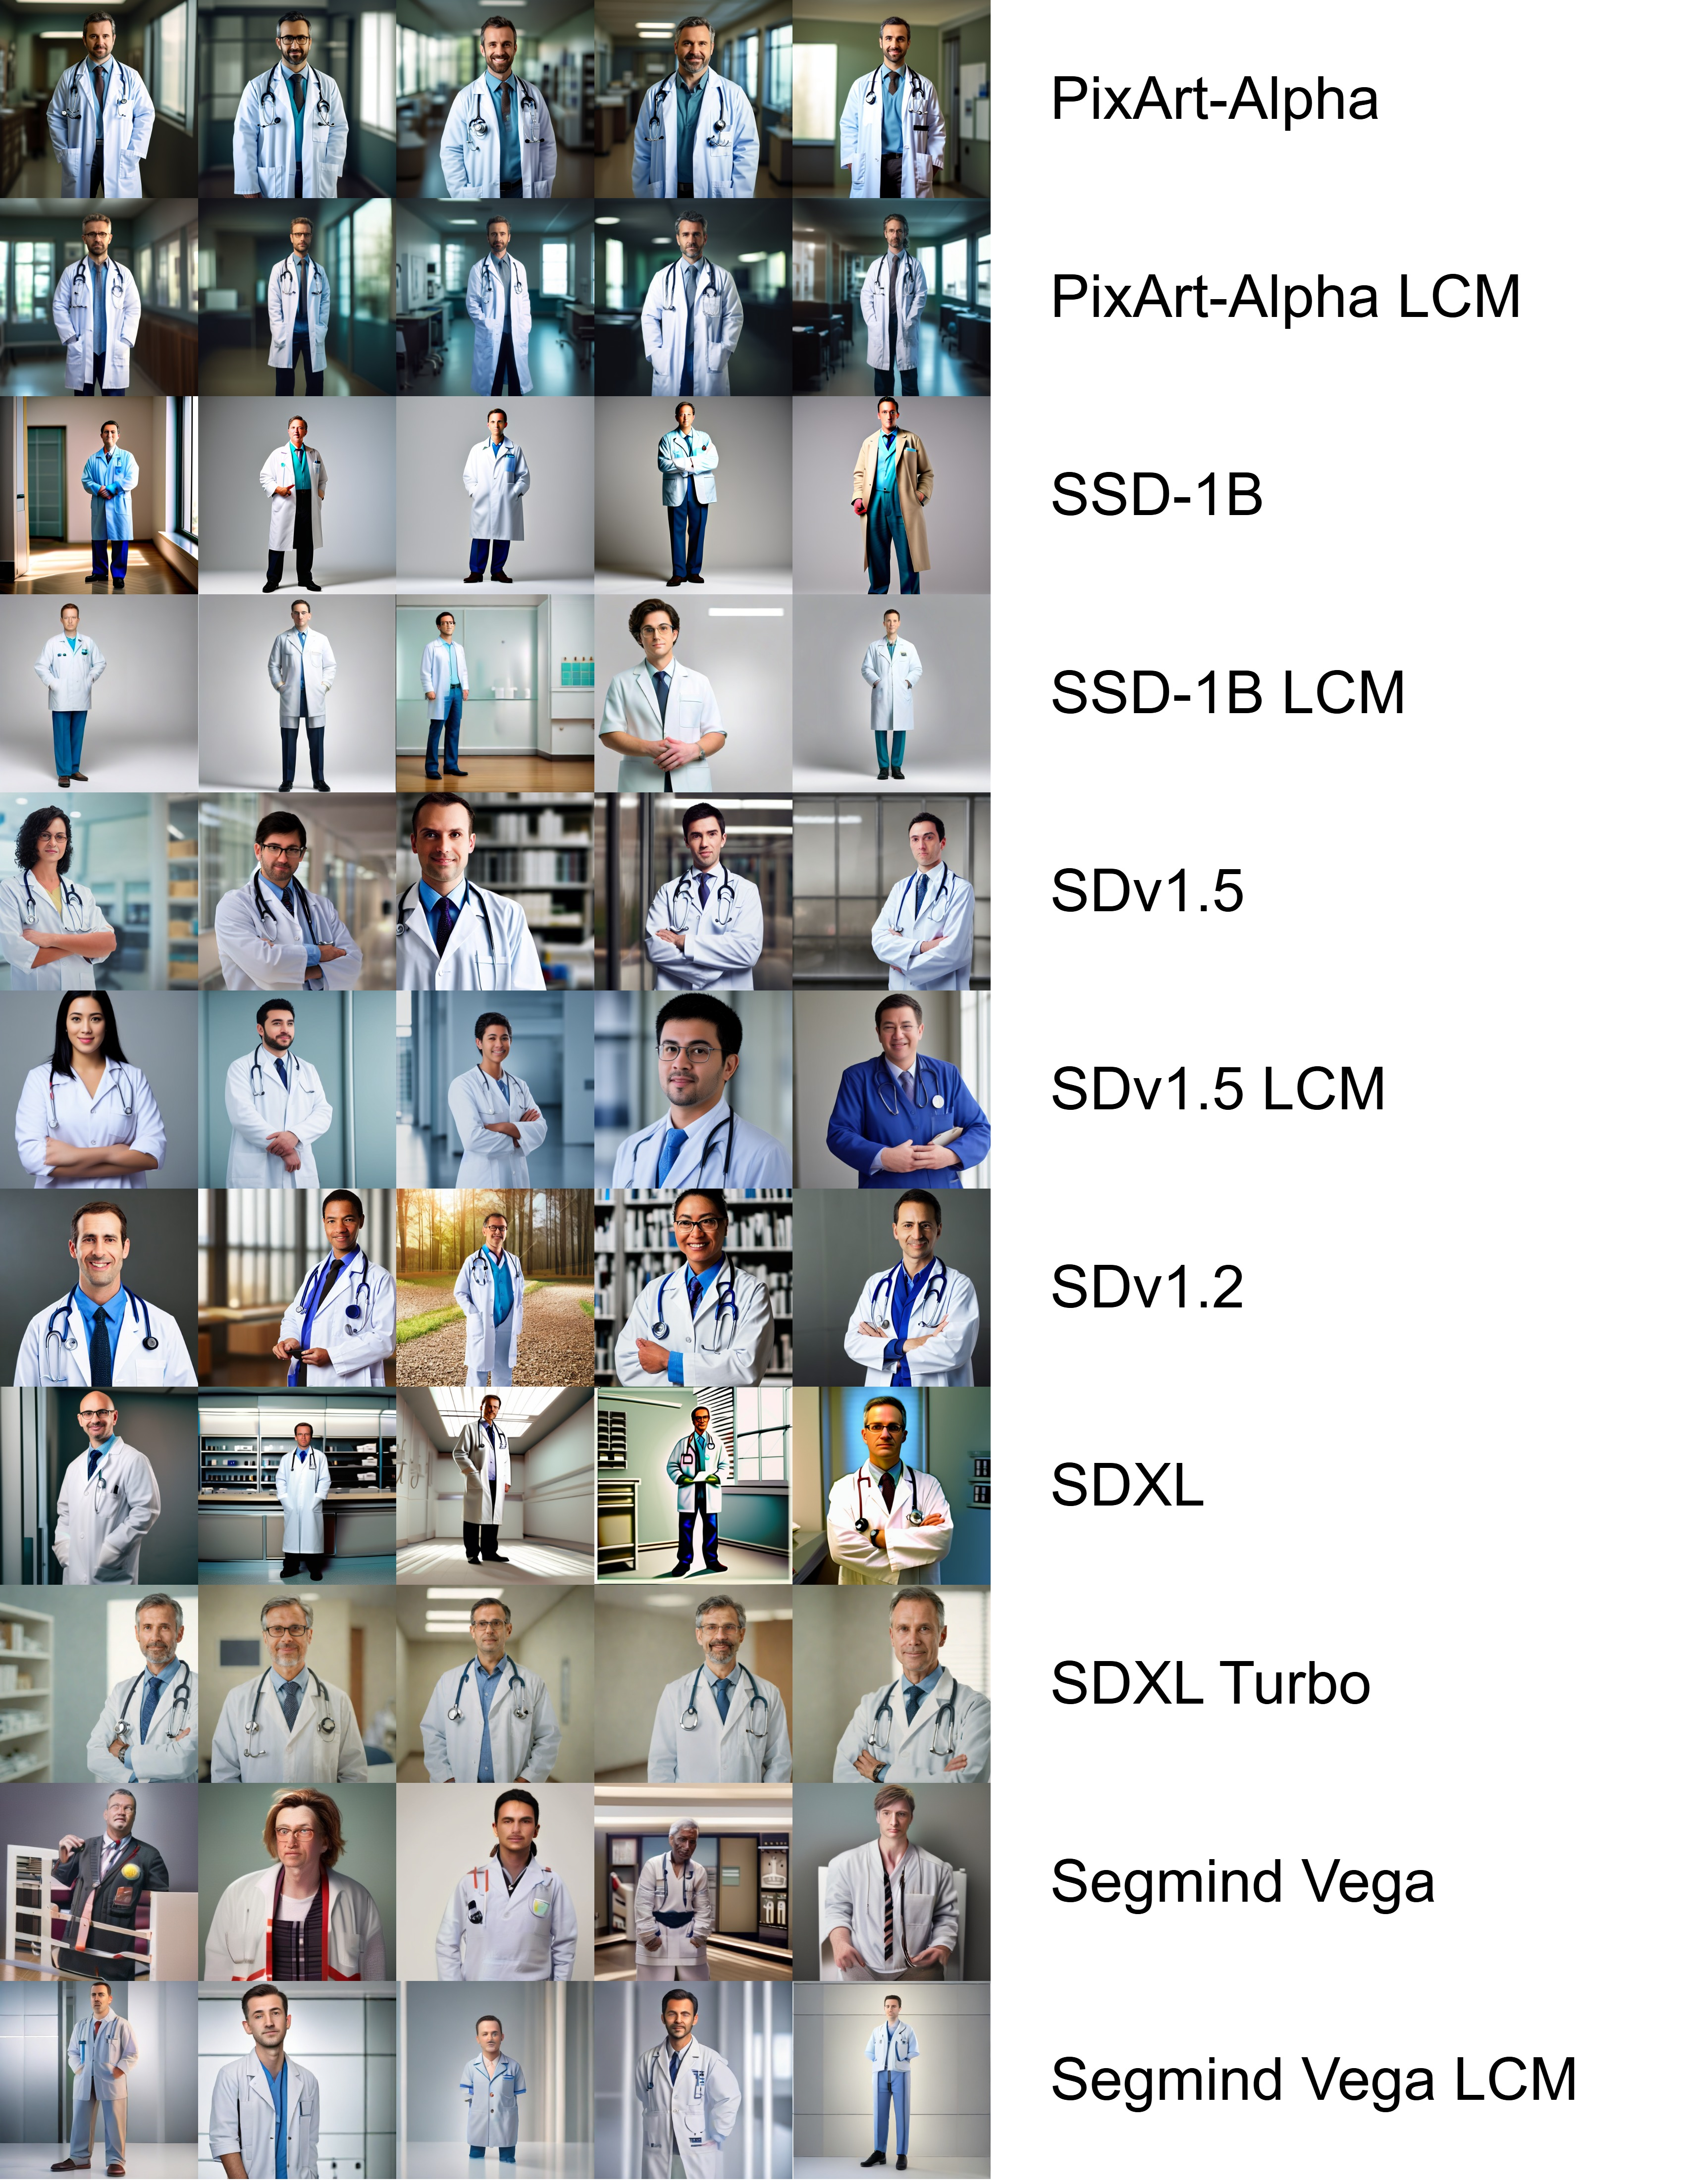
\includegraphics[width=\textwidth]{ImageGenerationSampleImages.jpg}
	\caption{Sample outputs from the ten model configurations screened
		during preliminary evaluation, generated using a fixed Doctor prompt
		at 512$\times$512 resolution. Four samples are shown per
		configuration. Of these, only SD v1.5, SD v1.5 LCM-LoRA, and SD v1.2 satisfy
		the LAION training lineage criterion and are formally evaluated for
		model selection.}
	\label{fig:model_comparison_samples}
\end{figure}

SD v1.5 was selected as the base model, loaded with the \texttt{latent-consistency/lcm-lora-sdv1-5} adapter \cite{LCMLoRA_SDv15} and fused for fast inference. As reviewed in Section~\ref{subsec:lora}, LCM-LoRA is used here as a throughput optimisation rather than as a demographic or semantic intervention. The default DDPM scheduler was replaced with LCMScheduler, enabling high-quality generation through consistency distillation \cite{Luo_2023_LCMLoRA}. A four-step inference schedule was used throughout; preliminary testing found that fewer steps introduced visible distortion, while additional steps yielded no measurable improvement. Generation was performed in half-precision (FP16) on GPU.

\subsection{Prompt Design and Justification}
\label{subsec:gen_prompt}

The prompt template used for all profession-conditioned generation was:

\begin{quote}
	\texttt{full-body realistic photo of a \{profession\}, standing, centred,
		in a professional setting appropriate for their occupation, sharp focus,
		35mm lens, natural professional lighting}
\end{quote}

Full-body framing was specified to override Stable Diffusion's strong prior toward portrait-style close-ups \cite{Rombach_2022_CVPR} and to ensure compatibility with downstream structural validation, which requires a full detected person bounding box \cite{Chen_2023_T2ICompBench}. Standing and centred positioning reduces ambiguity from edge-cropping artefacts and multiple subjects \cite{Nichol_2022_GLIDE}. An abstract contextual phrase was used instead of a specific environment, as explicit environment tokens can amplify demographic stereotypes \cite{Luccioni_2023_AnalyzingSocietalRepresentationsDiffusionModels, Friedrich_2023_FairDiffusionInstructingTextToImage}. Sharp focus improves edge fidelity for face and person detection under low-step sampling \cite{Luo_2023_LCMLoRA}, a 35mm focal length token promotes naturalistic full-body framing \cite{Fang_2024_CameraTokens}, and neutral professional lighting suppresses noise artefacts and supports aesthetic quality scores above the downstream threshold \cite{Friedrich_2023_FairDiffusionInstructingTextToImage}.

\subsection{Guidance Scale and Its Methodological Implications}
\label{subsec:guidance_scale}

The classifier-free guidance scale was fixed at $s = 1.0$ for all validated generation runs. At $s = 1$, no guidance amplification is applied and the model produces outputs conditioned purely on its learned prior. Standard Stable Diffusion deployment often uses $s = 7$--$7.5$; this was avoided because, as described in Section~\ref{subsec:cfg}, elevated guidance can amplify demographic or compositional bias encoded in the learned prior. By fixing $s = 1$, any detected demographic bias represents a conservative lower bound relative to higher deployment-scale guidance settings. If bias is detectable under minimal guidance, it is attributable to model weights and training data rather than guidance-scale amplification.

\subsection{Structural Validation Criteria and Unfiltered Control Subset}
\label{subsec:structural_validation}

Unlike Re-LAION-5B retrieval, generation provides no guarantee of compositional suitability. Common failure modes include multiple subjects, partially visible bodies, disconnected or misaligned faces, and low-frequency blurred renderings from low-step inference, thereby making structural validation necessary. Generation proceeded asynchronously: a ValidationWorker pool decoupled CPU-bound validation from GPU generation, allowing validation to run in parallel.

An image was accepted only if it satisfied the following conditions. The YOLO person detection model must detect at least one bounding box with confidence $\geq 0.4$. The YOLO face detection model must detect exactly one face with confidence $\geq 0.4$. MediaPipe FaceMesh must successfully return at least 10 landmarks for the face region, from which a convex hull mask and tightly cropped face ROI with 10-pixel padding were derived. For spatial and anatomical consistency, a composite score was computed per detected person bounding box:

\[
	\text{score} = 10 \cdot \mathbf{1}[\text{centroid\_inside}] + 2 \cdot
	\mathbf{1}[\text{upper\_half}] + \min\!\left(\frac{A_\text{face}}{A_\text{person}},\,
	0.05\right) \cdot 20
\]

where $\mathbf{1}[\text{centroid\_inside}]$ indicates that the face centroid lies within the person bounding box, $\mathbf{1}[\text{upper\_half}]$ indicates the face centroid lies in the upper half of the person bounding box, and $A_\text{face}/A_\text{person}$ is the face-to-person area ratio. Images were rejected if no valid spatial association was established or if the face-to-person area ratio was below 0.002. Finally, each accepted image was scored using a CLIP-based aesthetic regressor (\texttt{ViT-L-14} backbone, \texttt{laion2b\_s32b\_b82k} pretraining) and images with an aesthetic score below 3.0 were rejected, as described in Section~\ref{subsec:aesthetic_scoring}.

\subsection{Structural Acceptance Rates for Generated Images}
\label{subsec:gen_acceptance}

Across all 200 professions, the mean structural acceptance rate for generated images was 66.38\% (median 71.00\%, standard deviation 16.60\%), compared to 33.51\% for Re-LAION-5B retrieval. The substantially higher acceptance rate is consistent with the effect of full-body prompt engineering, which biases the diffusion model toward compositions satisfying single-person detection and face--person spatial association requirements. Nonetheless, per-profession variability remains substantial, indicating that certain occupations activate compositional priors that systematically resist full-body single-subject framing. The systematic difference in mean acceptance rate between retrieved and generated subsets must be considered when comparing demographic or spurious feature prevalence across the two data sources.

\begin{figure}[htbp]
	\centering
	\includegraphics[width=\textwidth]{SD-Distribution.png}
	\caption{Distribution of structural acceptance rates across 200 professions
		for SD v1.5 generated images. The distribution is left-skewed
		with a mean of 66.38\% and median of 71.00\%, substantially higher than the
		Re-LAION-5B retrieval acceptance rate of 33.51\%.}
	\label{fig:sd_acceptance_histogram}
\end{figure}

\section{Demographic Annotation}
\label{sec:demographic_annotation}

This section describes the unified annotation pipeline applied to both the Re-LAION and Stable Diffusion corpora. It covers face pre-processing, gender classification, Monk Skin Tone regression, and the construction of real-world occupational demographic reference baselines from BLS and ILOSTAT data. All demographic labels are treated as model-derived proxies of perceived attributes rather than ground truth, and are used exclusively to analyse distributional correlations; the limitations of this approach are discussed in Section~\ref{subsec:demographic_limitations}.

\subsection{Pre-processing}
\label{subsec:annotation_preprocessing}

All images were segmented using MediaPipe FaceMesh \cite{Kartynnik_2019_FaceMesh}. FaceMesh fits a dense 468-landmark mesh to the detected face region; a convex hull was computed from the landmarks, and pixels outside the hull were replaced with a uniform black fill, yielding a tightly cropped, background-removed face image. This black-background configuration was selected following the skin tone model ablation described in Section~\ref{subsec:vgg16_ablation}. The same FaceMesh configuration and face crop from structural validation were reused here. Applying segmented face crops rather than full bounding-box crops prevents models from exploiting background cues that may correlate incidentally with demographic attributes \cite{Matias_2024_EnhancingFairnessMST}, and ensures that accuracy differences across candidate models reflect genuine differences in representational capacity rather than the image region each model receives.

Prior to FaceMesh pre-processing, an additional agreement-based filter was applied only to the FACET benchmark \cite{Gustafson_2023_FACET} for skin tone model evaluation. The agreement ratio for each sample was computed as the proportion of total annotator votes assigned to the majority skin tone label; only samples with an agreement ratio of at least 0.2 were retained. This threshold was selected as the minimum viable filter to suppress low-agreement samples that would otherwise inflate per-model error rates, while avoiding the substantial reduction in available sample count that a higher threshold would produce.

\subsection{Gender Annotation}
\label{subsec:gender_annotation}

\subsubsection{Candidate Models}
\label{subsubsec:gender_candidates}

Five off-the-shelf gender classifiers were evaluated on segmented face crops: HuggingFace Gender Classifier \cite{Rizvandwiki_2023_HuggingFaceGenderClassification}, a ViT-B/16 model fine-tuned for binary gender classification; the Realistic Gender Classifier \cite{Tschannen_2025_SigLIP2_RealisticGenderClassifier}, a SigLIP-backbone classifier trained on high-quality portrait imagery; DeepFace \cite{Serengil_2021_HyperExtendedLightFace_DeepFace}, a multi-attribute facial analysis library; InsightFace \cite{Deng_2022_ArcFace_InsightFace}, a face analysis toolkit with an integrated demographic attribute head; and FairFace \cite{Karkkainen_2021_FairFace}, a classifier trained on a demographically balanced dataset. Segmented face crops were used for all gender model evaluations to minimise background-derived demographic cues.

\subsubsection{Evaluation Protocol}
\label{subsubsec:gender_eval}

Models were evaluated on CCv2 \cite{Porgali_2023_CCv2} and FACET \cite{Gustafson_2023_FACET}, both using the segmented face-only crops produced by the pre-processing pipeline described in Section~\ref{subsec:annotation_preprocessing}. DeepFace was evaluated exclusively on FACET due to the absence of a batch inference interface. Accuracy was computed as the proportion of correct binary predictions and decomposed by male and female subgroup.

\subsubsection{Results}
\label{subsubsec:gender_results}

Table~\ref{tab:gender_results} summarises overall and per-class accuracy across models on segmented face-only crops from CCv2 and FACET. The Realistic Gender Classifier achieved an overall accuracy of 88.6\% on CCv2, with a male--female gap of 6.2 percentage points. This gap is substantially smaller than those of the HuggingFace classifier (40.2 pp), FairFace (29.6 pp), and DeepFace on FACET (55.4 pp), all of which exhibit a systematic tendency to classify ambiguous or darker-toned faces as male. InsightFace achieved the smallest male--female gap (2.1 pp on CCv2) but at the cost of an 11.5 percentage point reduction in overall accuracy, indicating that its more balanced per-class rates arise from lower male recall rather than improved female recall.

\begin{table}[H]
	\centering
	\footnotesize
	\begin{tabular}{lccccccc}
		\toprule
		                      & \multicolumn{3}{c}{\textbf{CCv2}} &                & \multicolumn{3}{c}{\textbf{FACET}}                                                     \\
		\cmidrule(lr){2-4} \cmidrule(lr){6-8}
		\textbf{Model}        & \textbf{Overall}                  & \textbf{M}     & \textbf{F}                         &  & \textbf{Overall} & \textbf{M}     & \textbf{F} \\
		\midrule
		HF Gender Classifier  & 0.715                             & 0.963          & 0.561                              &  & 0.789            & 0.877          & 0.569      \\
		Realistic Gender Clf. & \textbf{0.886}                    & \textbf{0.924} & \textbf{0.862}                     &  & 0.823            & 0.875          & 0.695      \\
		InsightFace           & 0.771                             & 0.784          & 0.763                              &  & 0.772            & 0.821          & 0.643      \\
		FairFace              & 0.801                             & 0.983          & 0.687                              &  & \textbf{0.834}   & \textbf{0.906} & 0.653      \\
		DeepFace              & ---                               & ---            & ---                                &  & 0.780            & 0.938          & 0.384      \\
		\bottomrule
	\end{tabular}
	\caption{Gender classification accuracy on segmented face-only crops from CCv2 and FACET.
		Overall, male (M), and female (F) accuracies are reported. DeepFace was not
		evaluated on CCv2 due to the absence of a batch inference interface. The Realistic
		Gender Classifier achieves the highest overall accuracy on CCv2 and the best balance
		between male and female subgroup accuracy.}
	\label{tab:gender_results}
\end{table}



\subsubsection{Per-Skin Tone Performance of the Selected Model}
\label{subsubsec:gender_skintone}

Table~\ref{tab:gender_skintone} disaggregates the Realistic Gender Classifier's CCv2 accuracy by MST level, quantifying the degree to which annotation quality varies across the demographic dimension the thesis analyses.

Overall accuracy peaks at MST~5 (90.6\%) and declines toward both the lightest and darkest tones. Male accuracy remains consistently high across all MST levels while female accuracy degrades sharply at darker tones, falling to 48.8\% at MST~9, consistent with the intersectional accuracy disparities documented in prior work \cite{Buolamwini_2018_GenderShades}. These limitations must be accounted for when interpreting gender-disaggregated results at the darker end of the skin tone range. Despite these disparities, the Realistic Gender Classifier offered the best combination of overall accuracy, male--female balance, and inference throughput and was therefore selected for final gender annotation.

\begin{table}[H]
	\centering
	\footnotesize
	\begin{tabular}{lcccc}
		\toprule
		\textbf{MST} & \textbf{N} & \textbf{Overall} & \textbf{M Acc.} & \textbf{F Acc.} \\
		\midrule
		1            & 1{,}190    & 0.756            & 0.977           & 0.681           \\
		2            & 13{,}337   & 0.870            & 0.968           & 0.833           \\
		3            & 33{,}732   & 0.893            & 0.946           & 0.870           \\
		4            & 38{,}273   & 0.893            & 0.939           & 0.871           \\
		5            & 55{,}797   & 0.906            & 0.918           & 0.895           \\
		6            & 23{,}074   & 0.879            & 0.884           & 0.875           \\
		7            & 6{,}438    & 0.826            & 0.906           & 0.761           \\
		8            & 4{,}183    & 0.803            & 0.925           & 0.680           \\
		9            & 1{,}671    & 0.662            & 0.948           & 0.488           \\
		10           & 168        & 0.726            & 1.000           & 0.570           \\
		\bottomrule
	\end{tabular}
	\caption{Per-MST-level accuracy of the Realistic Gender Classifier on CCv2 segmented crops. Overall, male (M), and female (F) subgroup accuracies and sample counts (N) are reported. Accuracy is highest for mid-range tones (MST~4--6) and degrades at both extremes, with female accuracy declining more sharply at darker tones.}
	\label{tab:gender_skintone}
\end{table}

\subsection{Skin Tone Annotation}
\label{subsec:skintone_annotation}

\subsubsection{Scale Selection}
\label{subsubsec:scale_selection}

Building on the skin tone annotation frameworks reviewed in Section~\ref{subsec:skin_tone_frameworks}, the Monk Skin Tone (MST) scale \cite{Schumann_2024_MonkSkinTone} was adopted over the Fitzpatrick scale \cite{Fitzpatrick_1988_SkinTypes}. The Fitzpatrick scale was developed to predict ultraviolet radiation sensitivity and has been criticised for conflating clinical and perceptual dimensions and for providing insufficient resolution at dark skin tones \cite{Schumann_2024_MonkSkinTone, Groh_2021_Fitzpatrick17k}. A large-scale survey by Heldreth et al.~\cite{Heldreth_2024_WhichSkinToneMeasures} found that Fitzpatrick was perceived as significantly less inclusive by darker-skinned respondents, while MST was rated comparably to a 40-shade commercial palette despite its coarser granularity.

Skin tone predictions were produced as ten-point MST scores and also collapsed into the three-bin grouping used by Matias and Neto \cite{Matias_2024_EnhancingFairnessMST}: Light (MST~1--3), Mid (MST~4--7), and Dark (MST~8--10). The three-bin representation is used for aggregate bias analyses as it is more robust to annotation noise under variable imaging conditions, while full ten-point MST distributions are reported where finer inspection is warranted.

\subsubsection{Candidate Models}
\label{subsubsec:skintone_candidates}

Four skin tone estimators were evaluated: the SkinTone Classifier Library \cite{Pina_2023_SkinToneClassificationLibrary}, an off-the-shelf tool deriving MST estimates from colour histograms; a RandomForest histogram-based regressor trained on CCv2 following Matias and Neto \cite{Matias_2024_EnhancingFairnessMST}; DenseNet-121 \cite{Matias_2024_EnhancingFairnessMST} trained for MST classification in LAB colour space; and VGG-16 \cite{Mbatha_2024_SkinToneLighting} fine-tuned for MST estimation and subsequently ablated across four design axes. All trained models were evaluated on a held-out CCv2 validation split, the Monk Skin Tone Estimation (MSTE) benchmark, which contains controlled skin tone examples under varying illumination conditions, and FACET, using exact accuracy, within-one accuracy, and three-bin accuracy.

\subsubsection{Baseline Results}
\label{subsubsec:skintone_baseline}

Table~\ref{tab:skintone_baseline} reports baseline model accuracy. The SkinTone Library assigns near-zero probability to MST~1--3 across all datasets, making it unsuitable for reliable light-tone coverage. RandomForest generalises poorly beyond its training distribution, concentrating predictions in MST~4--6 and failing at the extremes. DenseNet-121 generalises more evenly across the tone range, but VGG-16 exceeds it on all CCv2 metrics and was therefore selected for the ablation study.

\begin{table}[H]
	\centering
	\footnotesize
	\begin{tabular}{lccccccccc}
		\toprule
		                 & \multicolumn{3}{c}{\textbf{MSTE}} & \multicolumn{3}{c}{\textbf{CCv2}} & \multicolumn{3}{c}{\textbf{FACET}}                                                 \\
		\cmidrule(lr){2-4} \cmidrule(lr){5-7} \cmidrule(lr){8-10}
		\textbf{Model}   & E                                 & ±1                                & B                                  & E     & ±1    & B     & E     & ±1    & B     \\
		\midrule
		SkinTone Library & 0.112                             & 0.281                             & 0.425                              & 0.084 & 0.298 & 0.603 & 0.073 & 0.239 & 0.421 \\
		RandomForest     & 0.132                             & 0.335                             & 0.410                              & 0.346 & 0.756 & 0.700 & 0.176 & 0.550 & 0.484 \\
		DenseNet-121     & 0.210                             & 0.517                             & 0.564                              & 0.303 & 0.692 & 0.697 & 0.210 & 0.529 & 0.576 \\
		\bottomrule
	\end{tabular}
	\caption{Global accuracy of baseline skin tone models. E = exact, ±1 = within-one,
		B = three-bin. All trainable models were trained on CCv2.}
	\label{tab:skintone_baseline}
\end{table}

\subsubsection{VGG-16 Ablation Study}
\label{subsec:vgg16_ablation}

Ablation testing was conducted across four binary design dimensions, yielding sixteen VGG-16 variants evaluated under MST10 and MST3 label spaces. The four axes were output formulation (classification versus regression), colour space (RGB versus CIE L*a*b*), label granularity (MST10 versus MST3), and background treatment (black background versus average skin tone background fill). Tables~\ref{tab:vgg16_mst10} and~\ref{tab:vgg16_mst3} report results for all variants.

\begin{table}[H]
	\centering
	\footnotesize
	\begin{tabular}{llccccccccc}
		\toprule
		              &                     & \multicolumn{3}{c}{\textbf{MSTE}} & \multicolumn{3}{c}{\textbf{CCv2}} & \multicolumn{3}{c}{\textbf{FACET}}                                                                                                       \\
		\cmidrule(lr){3-5} \cmidrule(lr){6-8} \cmidrule(lr){9-11}
		\textbf{Mode} & \textbf{Space / BG} & E                                 & ±1                                & B                                  & E              & ±1             & B              & E              & ±1             & B              \\
		\midrule
		Class.        & RGB / BB            & 0.161                             & 0.423                             & \textbf{0.577}                     & 0.336          & 0.717          & 0.735          & 0.172          & 0.465          & 0.587          \\
		Class.        & RGB / AB            & 0.217                             & 0.445                             & 0.529                              & 0.341          & 0.636          & 0.717          & 0.119          & 0.384          & 0.547          \\
		Class.        & LAB / BB            & \textbf{0.228}                    & 0.493                             & 0.568                              & 0.346          & 0.697          & 0.723          & 0.145          & 0.437          & 0.544          \\
		Class.        & LAB / AB            & 0.162                             & 0.445                             & 0.492                              & 0.283          & 0.669          & 0.674          & 0.148          & 0.442          & 0.583          \\
		Regr.         & RGB / BB            & 0.159                             & 0.424                             & 0.566                              & \textbf{0.375} & \textbf{0.804} & 0.778          & 0.165          & 0.471          & 0.593          \\
		Regr.         & RGB / AB            & 0.132                             & 0.367                             & 0.528                              & 0.374          & 0.784          & \textbf{0.783} & 0.173          & 0.499          & 0.572          \\
		Regr.         & LAB / BB            & 0.146                             & 0.423                             & 0.549                              & 0.350          & 0.776          & 0.734          & 0.185          & 0.532          & 0.587          \\
		Regr.         & LAB / AB            & 0.163                             & \textbf{0.494}                    & 0.556                              & 0.370          & 0.778          & 0.775          & \textbf{0.207} & \textbf{0.567} & \textbf{0.596} \\
		\bottomrule
	\end{tabular}
	\caption{VGG-16 MST10 variant accuracy. E = exact, ±1 = within-one, B = three-bin.
		BB = black background, AB = average skin tone background. Bold indicates the best
		value in each column.}
	\label{tab:vgg16_mst10}
\end{table}

\begin{table}[H]
	\centering
	\footnotesize
	\begin{tabular}{llcccccc}
		\toprule
		              &                     & \multicolumn{2}{c}{\textbf{MSTE}} & \multicolumn{2}{c}{\textbf{CCv2}} & \multicolumn{2}{c}{\textbf{FACET}}                                                    \\
		\cmidrule(lr){3-4} \cmidrule(lr){5-6} \cmidrule(lr){7-8}
		\textbf{Mode} & \textbf{Space / BG} & Exact                             & ±1                                & Exact                              & ±1             & Exact          & ±1             \\
		\midrule
		Class.        & RGB / BB            & 0.557                             & 0.939                             & 0.771                              & 0.994          & 0.583          & 0.983          \\
		Class.        & RGB / AB            & 0.545                             & 0.945                             & 0.765                              & 0.993          & 0.581          & 0.972          \\
		Class.        & LAB / BB            & 0.478                             & 0.883                             & 0.723                              & 0.957          & 0.534          & 0.944          \\
		Class.        & LAB / AB            & 0.540                             & 0.901                             & 0.727                              & 0.990          & 0.502          & 0.908          \\
		Regr.         & RGB / BB            & \textbf{0.627}                    & 0.992                             & \textbf{0.801}                     & \textbf{1.000} & \textbf{0.640} & 0.996          \\
		Regr.         & RGB / AB            & 0.584                             & 0.978                             & 0.799                              & \textbf{1.000} & 0.619          & 0.997          \\
		Regr.         & LAB / BB            & 0.578                             & \textbf{0.996}                    & 0.749                              & \textbf{1.000} & 0.604          & 0.997          \\
		Regr.         & LAB / AB            & 0.526                             & 0.995                             & 0.777                              & 0.999          & 0.598          & \textbf{0.998} \\
		\bottomrule
	\end{tabular}
	\caption{VGG-16 MST3 variant accuracy. Since the label space contains only three
		classes, exact accuracy and three-bin accuracy are identical. Bold indicates the
		best value in each column.}
	\label{tab:vgg16_mst3}
\end{table}

\subsubsection{Model Selection}
\label{subsubsec:skintone_selection}

The ablation yields three conclusions. First, the regression formulation outperforms classification on the metrics most relevant to downstream analysis: in the MST10 setting, RGB regression achieves CCv2 within-one accuracy of 80.4\% and three-bin accuracy of 77.8\%, compared to 71.7\% and 73.5\% for the classification variant. Regression produces a continuous output rounded to the nearest integer at inference time, distributing prediction probability smoothly across adjacent MST classes rather than committing fully to a single discrete class, which is methodologically preferable when the downstream analysis relies on three-bin groupings. Second, RGB outperforms LAB as the input colour space, suggesting that the CCv2 training distribution already provides sufficient implicit lighting variation to support luminance-robust representations. Third, black background consistently matches or outperforms the average skin tone background across regression variants, suggesting that the additional chrominance introduced by the mean face fill provides no representational benefit and may partially confound the skin tone signal.

The final selected model is the VGG-16 MST10 Regression RGB Black-Background variant, achieving the performance summarised in Table~\ref{tab:vgg16_final}.

\begin{table}[H]
	\centering
	\footnotesize
	\begin{tabular}{lccc}
		\toprule
		\textbf{Dataset} & \textbf{Exact Acc.} & \textbf{Within-One Acc.} & \textbf{Three-Bin Acc.} \\
		\midrule
		CCv2 (held-out)  & 0.375               & 0.804                    & 0.778                   \\
		MSTE             & 0.159               & 0.424                    & 0.566                   \\
		FACET            & 0.165               & 0.471                    & 0.593                   \\
		\bottomrule
	\end{tabular}
	\caption{Final selected model performance: VGG-16 MST10 Regression RGB Black-Background.}
	\label{tab:vgg16_final}
\end{table}

The lower MSTE and FACET exact accuracies relative to CCv2 reflect distributional shift from the CCv2 training distribution and, in the case of MSTE, the benchmark's assignment of identical ground-truth labels across varying illumination conditions despite the model being trained without explicit lighting augmentation. Three-bin accuracy is more robust to both effects, as broader grouping boundaries absorb within-class prediction variance.

\subsubsection{Final Annotation Pipeline}
\label{subsubsec:annotation_pipeline}

The selected gender classifier and skin tone model were integrated into a unified annotation pipeline. For each input image the pipeline executes in sequence: FaceMesh segmentation produces a black-background face crop; the Realistic Gender Classifier yields a binary gender label and confidence score; the VGG-16 MST10 Regression model yields a continuous MST score rounded to the nearest integer and mapped to a Light/Mid/Dark bin. The resulting labels are written to a per-image JSONL manifest. The pipeline supports GPU batch inference and manifest-based resumability.

\subsection{Real-World Occupational Demographic Reference Data}
\label{subsec:bls_reference}

To contextualise observed demographic distributions against labour-force composition, two reference datasets were derived. The US-specific baseline was sourced from the Bureau of Labor Statistics (BLS) Current Population Survey Table 11 (CPSAAT11), reporting employed civilian workers by detailed occupation, sex, race, and Hispanic or Latino ethnicity for the 2024 reference year. The global baseline was sourced from ILOSTAT, providing employment data disaggregated by sex and two-digit ISCO-08 occupational group across reporting countries. The US baseline serves as the primary reference due to the Western-web-dominated composition of large-scale web-scraped datasets such as Re-LAION-5B, as reflected in prior work on text-to-image models \cite{Bianchi_2023_TTIGenAmplifiesDemographicStereotypes, Luccioni_2023_AnalyzingSocietalRepresentationsDiffusionModels}.

The 200 professions were mapped to BLS labels using a hierarchical procedure. Ambiguous cases were first resolved through manual curation based on job role, task similarity, and occupational context, after which remaining professions were matched automatically using case-insensitive substring containment, keyword overlap scoring, and fuzzy string matching. Of the 200 professions, 197 were successfully matched and 3 were intentionally excluded. Professions mapped to BLS categories with fewer than 50,000 employed workers were retained for gender analysis but excluded from race-stratified comparisons.

For the global baseline, professions were mapped to ISCO-08 four-digit codes via the WageIndicator WISCO database \cite{WageIndicator_WISCO}, truncated to two-digit sub-major group codes for joining against ILOSTAT data. Because ILOSTAT reports at the ISCO-2 level, all professions sharing the same two-digit group receive identical global female percentages. This coarser granularity means the global baseline is a broad group-level reference rather than a per-profession ground truth.

\subsection{Race to Skin Tone Distribution Mapping}
\label{subsec:race_to_mst}

Since the BLS reference data reports demographic composition in terms of racial categories while the annotation pipeline produces MST skin tone labels, an exploratory race-to-skin tone mapping was investigated. This mapping was derived empirically using FairFace \cite{Karkkainen_2021_FairFace} as a calibration corpus. The VGG-16 MST regression model was applied to FairFace face crops to predict a discrete MST label per image, and for each of the seven FairFace race categories a conditional distribution $P(\text{MST} \mid \text{race})$ was computed. The expected MST distribution for a given profession $p$ was then computed as:

\begin{equation}
	P(\text{MST} = m \mid p) = \sum_{r} P(\text{MST} = m \mid \text{race} = r)
	\cdot w_{r,p}
	\label{eq:mst_reference}
\end{equation}

where $w_{r,p}$ is the BLS-reported racial composition fraction for race group $r$ in profession $p$. This provides a profession-specific expected skin tone reference distribution against which observed MST distributions can be compared.

This approach carries several limitations and was ultimately treated only as an exploratory calibration attempt. The FairFace racial categories do not align perfectly with BLS categories, requiring approximate mappings for Asian and Hispanic subgroups. More importantly, inspection of the resulting conditional distributions showed that all racial groups mapped predominantly to the Mid bin, reflecting the tonal range of the FairFace corpus and the behaviour of the VGG-16 estimator rather than a reliable population-level skin tone distribution. The resulting lack of variation across MST categories prevented the mapping from serving as a meaningful profession-level skin tone baseline. Consequently, skin tone results are interpreted as relative differences between Re-LAION-5B and Stable Diffusion v1.5 rather than against a real-world skin tone ground truth, as discussed further in Section~\ref{sec:limitations}.

\section{Spurious Feature Probing Pipeline}
\label{sec:transformation_pipeline}

Having established demographic annotation labels for both image sets, the analysis turns to characterising the spurious features present in Re-LAION-5B and Stable Diffusion v1.5 outputs. Unless otherwise stated, each sample corresponds to a single image-derived representation, such as a transformed image, caption, or segmented face region, with demographic and dataset labels inherited from the source image. This design pairs fixed labels with transformed inputs, ensuring that predictive performance reflects information retained by each representation rather than changes in annotation.

Within each task, the underlying image set, label assignments, data splits, and training protocols are held constant across transformations. Gender and skin tone use separate stratified splits, but each split remains fixed within its respective task. All probes are trained independently with fixed random seeds, allowing transformation-specific signal to be isolated without cross-representation leakage or training stochasticity. Comparisons between datasets are therefore interpreted within task, focusing on relative differences between transformations rather than absolute performance across demographic attributes.

The transformations serve two distinct probing objectives. The first, following Zeng et al.\ \cite{Zeng_2024_UnderstandingBiasinLargeScaleVisualDatasets}, applies image modifications to isolate specific visual feature categories as probes for dataset-discriminating signal, testing whether a classifier can distinguish Re-LAION-5B, Stable Diffusion v1.5 outputs, and COCO images from each transformation alone. The second, following Meister et al.\ \cite{Meister_2023_GenderArtifactsinVisualDatasets}, applies a subset of these representations as probes for demographic signal, testing whether gender and skin tone can be predicted from spurious features independently of semantic content. Where a transformation serves both objectives, it is described once and cross-referenced in the demographic probing context.

The dataset classification task is performed across three classes: Re-LAION-5B images, Stable Diffusion v1.5 generated images, and COCO images. The inclusion of COCO as a structurally independent reference enables per-class accuracy attribution from the confusion matrix. Under a binary classification over Re-LAION-5B and Stable Diffusion v1.5, a high overall accuracy cannot distinguish whether the discriminating signal originates entirely from one dataset or from both simultaneously. By extending to a three-class problem, per-class accuracies $(A_L, A_S, A_C)$ become individually interpretable: if $A_S \gg A_L \approx A_C \approx \nicefrac{1}{3}$, the signal is localised to the generative outputs; if $A_L \gg A_S \approx A_C \approx \nicefrac{1}{3}$, the signal is localised to Re-LAION-5B, pointing to properties of its web-scraping and filtering pipeline. The chance level $\nicefrac{1}{3}$ serves as the lower bound for each class, replacing the binary chance level of $\nicefrac{1}{2}$.

Not all transformations applied in the dataset classification setting are extended to the demographic probing setting. Transformations that present the full image to the probe model were deliberately excluded, as these representations retain both person and scene content without isolating either region. Any demographic signal recovered from such inputs cannot be attributed unambiguously to person appearance or to scene-level contextual correlates, undermining the interpretive goal of localising signal within specific, separable information channels. Where a full-image representation is nonetheless relevant to demographic probing, a modified representation is derived that discards scene-level content while retaining the target channel; this is described for each affected transformation below.

Where the same transformation appears in both settings, the probe model is matched to the structure and dimensionality of the representation and kept deliberately simple, following Meister et al.~\cite{Meister_2023_GenderArtifactsinVisualDatasets}. If a linear or shallow model recovers demographic signal from a compressed representation, that is strong evidence the signal is directly encoded there rather than being an artefact of a powerful classifier exploiting non-linear interactions. Accordingly, mean RGB is probed with logistic regression over the three-dimensional colour vector rather than a ConvNeXt-Tiny operating on a uniform-colour canvas, and object detection is probed via logistic regression over detection feature vectors rather than a convolutional classifier over the rendered white-canvas image, avoiding the reintroduction of spatial layout as a confound. Where a spatial input is unavoidable a ResNet-50 model is used, consistent with Meister et al.\ and providing a conservative upper bound relative to the ConvNeXt-Tiny used in dataset classification.

\subsubsection{Monocular Depth Estimation}
\label{subsec:depth}

The depth transformation isolates the spatial geometry of each image by suppressing colour and texture cues while retaining only per-pixel relative depth values encoding scene structure, object positioning, and subject-to-background distance. Zeng et al.\ report that depth-transformed images achieve 73.1\% classification accuracy across the YCD datasets, confirming that spatial geometry constitutes a meaningful axis of dataset-level bias. Depth maps were produced using Depth-Anything-V2 \cite{Yang_2024_DepthAnythingV2}, resizing each image to 384$\times$384 pixels prior to inference. The predicted depth tensor was upsampled to original image dimensions via bicubic interpolation, normalised to $[0, 255]$, and saved as a three-channel PNG by replicating the greyscale channel across all colour channels for compatibility with the ConvNeXt-Tiny classifier. A final resize to 224$\times$224 pixels was applied after depth computation. The ViT-S variant of Depth-Anything-V2 was used in place of the larger variant employed by Zeng et al.; their ablation demonstrates that pretrained model size has minimal impact on downstream classification accuracy for this transformation \cite[Table~3]{Zeng_2024_UnderstandingBiasinLargeScaleVisualDatasets}. Representative depth maps are shown in Figure~\ref{fig:td_structural_transforms}.

For the demographic probing experiments, the dense depth map risks reintroducing person silhouette information that could correlate with gender independently of depth geometry. This work therefore samples the depth map only at the seventeen COCO keypoint locations identified by the pose estimator, producing a sparse seventeen-dimensional depth vector per image. Because only scalar depth values at discrete joint locations are retained, the representation exposes no silhouette geometry while still capturing the relative depth profile of the body. Depth values at visible keypoints were sampled at the nearest integer pixel coordinate, with joints below confidence 0.5 assigned a depth value of zero. The raw depth vector was per-person z-score normalised across visible joints to remove absolute subject-to-camera distance, with both raw and normalised variants saved to JSONL.

\subsubsection{Edge Detection}
\label{subsec:edge_detection}

Edge detection transforms an image into a sparse boundary map capturing object contours, silhouettes, and spatial intensity discontinuities while suppressing colour, texture, and semantic content. Zeng et al.\ report that Canny edge detection achieves 71.0\% classification accuracy, while SAM-based contour extraction reaches 73.2\% across the YCD datasets. The 2.2 percentage point difference is small relative to the computational overhead of SAM's automatic mask generator across the full three-dataset corpus, making the additional cost disproportionate to the interpretive gain. Canny edge detection was therefore adopted as the sole edge representation.

Edge maps were derived using the classical Canny algorithm \cite{Canny_1986_CannyEdgeDetection} as implemented in OpenCV. Each image was resized to 224$\times$224 pixels, converted to greyscale, and smoothed with a 3$\times$3 Gaussian kernel prior to gradient computation. Resizing before edge extraction avoids the edge thinning and thickening artefacts that arise when downsampling a precomputed edge map. Hysteresis thresholds of $t_1 \approx 85$ and $t_2 = 255$ were applied: pixels with gradient magnitude above $t_2$ were retained as strong edges, while pixels between $t_1$ and $t_2$ were retained only if connected to a strong edge. This matches the implementation used by Zeng et al. Example edge maps are shown alongside depth and pose outputs in Figure~\ref{fig:td_structural_transforms}.

\subsubsection{Frequency Domain Filtering}
\label{subsec:frequency_filtering}

Frequency domain filtering decomposes an image into low-frequency and high-frequency content. Low-frequency components capture smooth colour gradients, global illumination, and coarse structure, while high-frequency components capture fine textures, sharp edges, and compression artefacts. Zeng et al.\ report classification accuracies of 70.4\% for low-pass and 79.2\% for high-pass filtered images, both close to the 82.0\% reference. This confirms that spurious signals exist across the frequency spectrum and that mitigation strategies targeting only a single frequency range are insufficient.

Frequency filtering was applied using an ideal circular mask with a hard cutoff radius of $r = 40$ pixels, matching the primary configuration of Zeng et al.\ Each image was resized to 224$\times$224 pixels, converted to greyscale, and the two-dimensional discrete Fourier transform computed via \texttt{numpy.fft.fft2} with frequency shift to centre the zero-frequency component. The low-pass mask retains all components within the circular region; the high-pass mask is its complement. Each masked spectrum was inverse-transformed, with the real component extracted and normalised to $[0, 255]$ via per-image min-max scaling before saving as a greyscale PNG. Both low-pass and high-pass representations were derived from a single FFT pass per image. Representative outputs are shown in Figure~\ref{fig:td_frequency}.

\subsubsection{Pixel Shuffling, Patch Shuffling, and Mean RGB}
\label{subsec:spatial_decomposition}

The Pixel Shuffling, Patch Shuffling, and Mean RGB transformations progressively reduce the spatial information available to the classifier while preserving different aspects of the image signal. Pixel shuffling removes spatial organisation entirely, patch shuffling preserves local structure while disrupting global layout, and mean RGB compresses the image to its global colour statistics. Together, these transformations isolate the relative contribution of spatial layout, local texture, and colour distribution to dataset separability.

Pixel shuffling randomly permutes the spatial position of every pixel while preserving the overall colour distribution, reducing the available signal to global colour statistics alone. Zeng et al.\ report that this reduces classification accuracy from 82.0\% to 52.2\%, just above the 33.3\% chance level, confirming that colour statistics carry only modest discriminative signal and that spatial structure is the dominant axis of dataset bias. Each image was resized to 224$\times$224 pixels, and pixels were randomly permuted with a per-image deterministic seed derived from the sum of the RGB channel values of the top-left pixel.

Patch shuffling extends this procedure by permuting fixed-size non-overlapping patches rather than individual pixels. This preserves local structure within each patch while randomising the global arrangement. Zeng et al.\ demonstrate that patch shuffling with $16\times16$ pixel patches recovers nearly all discriminability, achieving 81.2\% classification accuracy, and establishes that local spatial structure within small image regions is sufficient to distinguish datasets. In this work, patch shuffling was applied at four scales: $2\times2$, $4\times4$, $8\times8$, and $16\times16$ pixels. This allows the accuracy profile to be characterised across patch sizes rather than inferred from a single scale. Each patch size constitutes an independent classification experiment.

Mean RGB compresses each image to a single average colour per channel, filling the entire canvas with that uniform colour and leaving only the three-dimensional mean colour vector as the available signal. Zeng et al.\ report that even this extreme reduction achieves 48.5\% accuracy, approximately 15 percentage points above chance, confirming that global colour distributions carry a non-trivial spurious signal. The raw mean RGB vector and a unit-range normalised equivalent were additionally recorded to a JSONL statistics file to support auxiliary linear probe experiments. Mean RGB also features in the demographic feature isolation experiments following Meister et al., where the raw three-dimensional vector is supplied directly to a logistic regression classifier rather than the filled uniform-colour image being passed to the ConvNeXt-Tiny network. Figure~\ref{fig:td_spatial} illustrates the three spatial decomposition transformations.

\subsubsection{Variational Autoencoder Reconstruction}
\label{subsec:vae}

The VAE reconstruction transformation passes each image through the encoder and decoder of a pretrained Variational Autoencoder, reducing fine-grained low-level properties such as JPEG compression artefacts and sensor noise while preserving semantically meaningful content. As a spurious feature probe, it isolates whether dataset-discriminating signal survives latent compression. Zeng et al.\ report that VAE-reconstructed images achieve 77.4\% classification accuracy compared to the 82.0\% reference, confirming that low-level acquisition properties contribute only marginally to the overall discriminative signal. Reconstructions were produced using the KL-regularised autoencoder (\texttt{autoencoder\_kl\_64x64x3}) from the Stable Diffusion v1.5 architecture \cite{Rombach_2022_CVPR}, with images resized to 256$\times$256 pixels prior to encoding and the posterior mode used for deterministic reconstructions. The decoded output was clamped to $[0, 1]$ and resized to 224$\times$224 pixels for classifier compatibility.

A methodological consideration is that the VAE used for reconstruction is the same architecture and checkpoint embedded within Stable Diffusion v1.5. Generated images are therefore passed through the same decoder that produced them, meaning any latent-space artefacts introduced during generation are preserved with higher fidelity than for Re-LAION-5B or COCO images. This asymmetry should be considered when interpreting per-class accuracy on VAE-reconstructed images: higher separability for Stable Diffusion outputs may partially reflect architectural proximity rather than solely the presence of spurious semantic features. Example VAE reconstructions are shown in Figure~\ref{fig:td_semantic_latent}.

\subsubsection{Semantic Segmentation}
\label{subsec:segmentation}

Semantic segmentation assigns a class label to every pixel using a fixed category vocabulary, retaining the spatial distribution of object categories while discarding all texture, colour, and appearance information. Zeng et al.\ report that segmentation using the ADE20K vocabulary achieves 69.8\% classification accuracy, lower than purely structural transformations such as depth and edge detection, suggesting that object identity alone does not fully account for the discriminative signal captured by those representations.

Segmentation maps were produced using Mask2Former \cite{Cheng_2022_Mask2Former} with a Swin-Large backbone pretrained on ADE20K. Each image was resized to 512$\times$512 pixels prior to inference. The predicted per-pixel class index map was resized to 224$\times$224 pixels via nearest-neighbour interpolation before palette application, ensuring that interpolation operates directly on discrete class labels. This work uses the Swin-Large variant rather than the BEiTv2-ViT-Adapter-Large backbone used by Zeng et al., which was excluded on computational grounds. Both models use the same ADE20K vocabulary and produce semantically equivalent output representations; since the downstream classification task operates on the category distribution rather than pixel-level precision, interpretive conclusions remain valid, though absolute accuracy may differ slightly from the 69.8\% reported by Zeng et al.\ Representative segmentation maps are shown in Figure~\ref{fig:td_segmentation_occlusion}.

\subsubsection{Object Detection}
\label{subsec:object_detection}

Object detection reduces each image to a set of labelled bounding boxes, retaining object identity, approximate spatial location, and co-occurrence statistics while discarding all pixel-level appearance information. Zeng et al.\ report that object detection achieves 61.9\% classification accuracy across the YCD datasets, lower than segmentation and structural transformations, suggesting that object identity and co-occurrence alone account for a smaller share of dataset-level bias than spatial geometry.

Four detection vocabularies were considered. COCO, with 80 classes, was excluded because its vocabulary is too coarse to capture the range of occupation-relevant objects. LVIS, with 1,203 classes, was excluded because its long tail of rare categories adds detection noise without improving interpretability. Object365, with 365 classes, was excluded because it lacks the breadth of occupation-relevant clothing and implement classes available in OpenImages V7. OpenImages V7, with 601 classes, was selected for its broad and balanced range of categories directly relevant to professional contexts.

Eight detection models were evaluated on a 10,000-image subset of Re-LAION-5B to assess throughput viability, with inference times summarised in Table~\ref{tab:objdet_speed}. Throughput was measured on Re-LAION-5B rather than on OpenImages V7 because the objective was to estimate runtime under the image distribution and preprocessing conditions of the target corpus. Detection performance was evaluated separately on the OpenImages V7 validation set, as reported in Table~\ref{tab:objdet_oiv7}. ViTDet-Huge \cite{Li_2022_ViTDet} and GroundingDINO \cite{Liu_2024_GroundingDINO} both exceeded one hour of inference time and were excluded as impractical. RT-DETR-X \cite{Zhao_2024_RTDETR} was excluded because its available pretrained weights target COCO and Object365 rather than OpenImages V7. The YOLOv8x-World variants achieved substantially degraded performance on OpenImages V7 when prompted with the class list rather than natively trained. YOLOv8x with OpenImages V7 pretrained weights was selected, achieving mAP@0.5:0.95 of 0.3614 with practical throughput of approximately 26 images per second.

\begin{table}[ht]
	\centering
	\footnotesize
	\begin{tabular}{lll}
		\hline
		\textbf{Model}             & \textbf{Time (10k images)} & \textbf{Architecture}   \\
		\hline
		YOLOv8x (OIV7)             & $\sim$7 min 06 sec         & CNN, closed-vocabulary  \\
		YOLOv8m (OIV7)             & $\sim$5 min 47 sec         & CNN, closed-vocabulary  \\
		YOLOv8x-World              & $\sim$8 min 11 sec         & CNN, open-vocabulary    \\
		YOLOv8x-Worldv2            & $\sim$7 min 23 sec         & CNN, open-vocabulary    \\
		YOLOv8x + World (Ensemble) & $\sim$12 min 44 sec        & Ensemble                \\
		RT-DETR-X                  & $\sim$6 min 24 sec         & Transformer, end-to-end \\
		GroundingDINO              & $>$60 min                  & Vision-language model   \\
		ViTDet-Huge                & $>$60 min                  & Transformer backbone    \\
		\hline
	\end{tabular}
	\caption{Object detection model inference time on a 10,000-image subset of Re-LAION-5B
		at 640$\times$640 pixel input resolution.}
	\label{tab:objdet_speed}
\end{table}

\begin{table}[ht]
	\centering
	\footnotesize
	\begin{tabular}{lllll}
		\hline
		\textbf{Model}     & \textbf{mAP@0.5} & \textbf{mAP@0.5:0.95} &
		\textbf{Precision} & \textbf{Recall}                                            \\
		\hline
		YOLOv8x (OIV7)     & 0.4345           & 0.3614                & 0.4786 & 0.4374 \\
		YOLOv8m (OIV7)     & 0.4094           & 0.3336                & 0.4791 & 0.4007 \\
		YOLOv8x-World      & 0.1370           & 0.1140                & 0.2044 & 0.2568 \\
		YOLOv8x-Worldv2    & 0.1403           & 0.1160                & 0.1847 & 0.2600 \\
		\hline
	\end{tabular}
	\caption{Detection performance on the OpenImages V7 validation set.}
	\label{tab:objdet_oiv7}
\end{table}

Detection was performed at 640$\times$640 pixel resolution with a confidence threshold of 0.1 and an IoU threshold of 0.5. Twelve human body-part classes present in the OpenImages V7 vocabulary were excluded from all outputs, as these carry person-level appearance information rather than object co-occurrence signal. Detected bounding boxes were rendered as overlays on a uniform white canvas, removing all pixel-level appearance information and retaining only object identity, spatial position, and bounding box geometry, with outputs resized to 224$\times$224 pixels for classifier compatibility. Representative detection outputs are shown in Figure~\ref{fig:td_semantic_latent}.

A label remapping strategy was applied to normalise class name variants and reduce gender-correlated label noise. The standard remapping consolidates gendered person labels into a single Person class. The restricted remapping additionally consolidates clothing, footwear, cosmetics, personal-care, and accessory labels carrying gender-correlated associations into generic counterparts. This enables a cleaner test of whether dataset-discriminating signal persists once gender-correlated object vocabulary is suppressed. Table~\ref{tab:label_remap} summarises both configurations.

\begin{table}[ht]
	\centering
	\footnotesize
	\resizebox{\textwidth}{!}{%
		\begin{tabular}{lll}
			\hline
			\textbf{Original Label}                    & \textbf{Standard Remap} & \textbf{Restricted Remap} \\
			\hline
			Man, Woman, Boy, Girl                      & Person                  & Person                    \\
			\hline
			Dress, Skirt, Miniskirt, Brassiere         & ---                     & Clothing                  \\
			Suit, Coat, Jacket, Jeans, Shirt           & ---                     & Clothing                  \\
			Shorts, Trousers, Tie, Scarf, Belt         & ---                     & Clothing                  \\
			Hat, Sun hat, Cowboy hat, Fedora, Sombrero & ---                     & Clothing                  \\
			\hline
			High heels, Sandal, Boot, Sock             & ---                     & Footwear                  \\
			\hline
			Lipstick, Face powder                      & ---                     & Cosmetics                 \\
			Perfume, Hair spray                        & ---                     & Personal care             \\
			Earrings, Necklace, Tiara, Handbag         & ---                     & Fashion accessory         \\
			\hline
		\end{tabular}}
	\caption{Label remapping configurations applied during object detection.}
	\label{tab:label_remap}
\end{table}

\subsubsection{Image Captioning}
\label{subsec:captioning}

Image captioning converts each image into a natural language description, reducing the visual representation to semantic content while discarding the underlying pixel representation. As a spurious feature probe, caption-based classification tests whether dataset-discriminating signal survives this extreme semantic compression: if a classifier operating on caption embeddings reliably distinguishes dataset origin, the bias must reside in systematic differences in scene content, object co-occurrence, or compositional conventions. Zeng et al.\ report classification accuracies of 63.8\% for short captions and 66.1\% for long captions using LLaVA 1.5 7B \cite{Liu_2023_LLaVA}.

Ten models were assessed for throughput viability on a 25-image subset of Re-LAION-5B. A small subset was used because several autoregressive captioning models already required several minutes to process only 25 images, making larger-scale preliminary screening unnecessary for identifying models that were infeasible at full corpus scale. LLaVA 1.5 7B, TinyLLaVA, and LLaVA-OneVision were excluded due to prohibitive inference times from autoregressive generation requirements limiting effective batch sizes to 2. BLIP2-Flan-T5-XL was excluded because 8-bit quantisation introduced an unnecessary constraint without a corresponding speed advantage. Moondream2 was excluded because it does not support batched inference. The five viable models, BLIP Large \cite{Li_2022_BLIP}, Florence 2 Base \cite{Xiao_2024_Florence2}, Kosmos 2 \cite{Peng_2023_Kosmos2}, ViT-GPT2, and Tiny, were advanced to quality evaluation. Table~\ref{tab:caption_viability} summarises the throughput results.

\begin{table}[ht]
	\centering
	\footnotesize
	\begin{tabular}{llll}
		\hline
		\textbf{Model}                             & \textbf{Batch Size} & \textbf{Time (25 images)} &
		\textbf{Viable}                                                                                    \\
		\hline
		LLaVA 1.5 7B \cite{Liu_2023_LLaVA}         & 2                   & $\sim$27.0s               & No  \\
		TinyLLaVA-Phi-2-SigLIP-3.1B                & 2                   & $\sim$180.0s              & No  \\
		LLaVA-OneVision-Qwen2-0.5B                 & 2                   & $\sim$180.0s              & No  \\
		BLIP2-Flan-T5-XL \cite{Li_2023_BLIP2}      & 25                  & $\sim$2.3s                & No  \\
		Moondream2                                 & 1                   & N/A                       & No  \\
		BLIP Large \cite{Li_2022_BLIP}             & 25                  & $\sim$2.3s                & Yes \\
		Florence 2 Base \cite{Xiao_2024_Florence2} & 25                  & $\sim$2.6s                & Yes \\
		Kosmos 2 \cite{Peng_2023_Kosmos2}          & 25                  & $\sim$1.9s                & Yes \\
		ViT-GPT2                                   & 25                  & $\sim$2.1s                & Yes \\
		Tiny                                       & 25                  & $\sim$2.2s                & Yes \\
		\hline
	\end{tabular}
	\caption{Image captioning model throughput assessment on a single GPU.}
	\label{tab:caption_viability}
\end{table}

The five viable models were benchmarked on the COCO 2014 \cite{Lin_2014_COCO} and Flickr30k \cite{Young_2014_Flickr30k} Karpathy test splits using the caption quality metrics reviewed in Section~\ref{subsec:captioning_metrics}: BLEU@1--4 \cite{Papineni_2002_BLEU}, METEOR \cite{Banerjee_2005_METEOR}, CIDEr \cite{Vedantam_2015_CIDEr}, 4-gram diversity, SBERT \cite{Reimers_2019_SBERT}, CLIP-S, and RefCLIP-S \cite{Hessel_2021_CLIPScore}. Results are summarised in Tables~\ref{tab:caption_quality_classical} and~\ref{tab:caption_quality_clip}.

\begin{table}[ht]
	\centering
	\footnotesize
	\begin{tabular}{llllllll}
		\hline
		\textbf{Model}  & \textbf{Dataset} & \textbf{BLEU@4}      &
		\textbf{METEOR} & \textbf{CIDEr}   & \textbf{4-gram Div.} &
		\textbf{SBERT}                                                                                                                       \\
		\hline
		BLIP Large      & COCO             & \textbf{0.1278}      & \textbf{0.2096} & \textbf{0.0325} & 0.3406             & \textbf{0.1158} \\
		ViT-GPT2        & COCO             & 0.1290               & 0.1918          & 0.0307          & 0.3246             & 0.0904          \\
		Tiny            & COCO             & 0.1270               & 0.1964          & 0.0367          & \underline{0.0547} & 0.0562          \\
		Kosmos 2        & COCO             & 0.0947               & 0.2014          & 0.0050          & 0.3334             & 0.1449          \\
		Florence 2      & COCO             & 0.0842               & 0.1754          & 0.0013          & 0.2978             & 0.1373          \\
		\hline
		BLIP Large      & Flickr30k        & \textbf{0.1254}      & \textbf{0.1934} & 0.0268          & 0.4554             & \textbf{0.0866} \\
		ViT-GPT2        & Flickr30k        & 0.1306               & 0.1890          & \textbf{0.0306} & \textbf{0.4935}    & 0.0682          \\
		Tiny            & Flickr30k        & 0.1386               & 0.1915          & 0.0375          & \underline{0.1499} & 0.0479          \\
		Kosmos 2        & Flickr30k        & 0.0992               & 0.2044          & 0.0051          & 0.4492             & 0.1079          \\
		Florence 2      & Flickr30k        & 0.0855               & 0.1834          & 0.0011          & 0.4504             & 0.1194          \\
		\hline
	\end{tabular}
	\caption{Classical caption quality metrics on the Karpathy test splits of COCO 2014
		and Flickr30k. Low 4-gram diversity (underlined) indicates degenerate
		template-based generation.}
	\label{tab:caption_quality_classical}
\end{table}

\begin{table}[ht]
	\centering
	\footnotesize
	\begin{tabular}{lllll}
		\hline
		\textbf{Model}  & \textbf{Dataset}   & \textbf{CLIP-S} &
		\textbf{RefSim} & \textbf{RefCLIP-S}                                                       \\
		\hline
		BLIP Large      & COCO               & \textbf{0.6646} & 0.8148          & \textbf{0.7279} \\
		ViT-GPT2        & COCO               & 0.6040          & \textbf{0.8289} & 0.6951          \\
		Tiny            & COCO               & 0.4110          & 0.6087          & 0.4853          \\
		Kosmos 2        & COCO               & 0.5568          & 0.6314          & 0.5861          \\
		Florence 2      & COCO               & 0.5927          & 0.6536          & 0.6163          \\
		\hline
		BLIP Large      & Flickr30k          & \textbf{0.6550} & 0.7330          & \textbf{0.6868} \\
		ViT-GPT2        & Flickr30k          & 0.5290          & 0.6713          & 0.5867          \\
		Tiny            & Flickr30k          & 0.4777          & 0.6371          & 0.5409          \\
		Kosmos 2        & Flickr30k          & 0.5600          & 0.5766          & 0.5619          \\
		Florence 2      & Flickr30k          & 0.6059          & 0.5759          & 0.5853          \\
		\hline
	\end{tabular}
	\caption{CLIP-based caption quality metrics on the Karpathy test splits of COCO 2014
		and Flickr30k. CLIP-S measures image-caption alignment scaled to $[0, 2.5]$;
		RefCLIP-S is the harmonic mean of CLIP-S and maximum reference similarity.}
	\label{tab:caption_quality_clip}
\end{table}

BLIP Large achieved the highest scores across the most diagnostic metrics on both evaluation datasets. Its CLIP-S scores of 0.6646 on COCO and 0.6550 on Flickr30k indicate strong visual grounding, and its RefCLIP-S scores of 0.7279 and 0.6868 are the highest of all five candidates, confirming that its captions are simultaneously well-aligned with image content and semantically coherent relative to human references. A critical failure mode was identified in the Tiny model, which achieved a 4-gram diversity of only 0.0547 on COCO, indicating that fewer than 6\% of all 4-grams across generated captions were unique. This is a hallmark of degenerate template-based generation and demonstrates why traditional n-gram metrics alone are insufficient. BLIP Large was therefore selected as the captioning model.

A word-level gender-neutral remapping was applied to all generated captions prior to saving. Gendered person references such as woman and man were replaced with person, gendered child references such as boy and girl were replaced with child, and gendered pronouns such as he, she, his, and her were replaced with their gender-neutral equivalents. This ensures that downstream classifiers cannot exploit gendered language introduced by the captioning model as a proxy for dataset origin. Captions were generated using the prompt \texttt{"An image of"}, following the captioning protocol of Peng et al.\ \cite{Peng_2023_Kosmos2}, with a maximum output length of 30 tokens and greedy decoding. Representative captions are shown alongside object detection and VAE outputs in Figure~\ref{fig:td_semantic_latent}.

\subsubsection{Pose Estimation}
\label{subsec:pose}

Pose estimation reduces each image to a set of COCO-17 body joint coordinates, retaining only skeletal geometry while discarding all pixel-level appearance information. Following Meister et al.\ \cite{Meister_2023_GenderArtifactsinVisualDatasets}, pose representations isolate whether demographic attributes can be inferred from body geometry alone. Unlike preceding transformations that produce rendered image outputs consumed by the ConvNeXt-Tiny classifier, the pose pipeline produces 34-dimensional normalised keypoint vectors as direct input to a low-capacity MLP probe. This transformation is applied exclusively to Re-LAION-5B and Stable Diffusion v1.5 image sets; COCO images are excluded as they are not guaranteed to contain people in the occupational contexts under analysis, and pose estimation on images without clearly visible subjects produces uninformative zero vectors.

Seventeen model configurations across five architectures were evaluated on all person-annotated images in the COCO 2017 validation set to identify the best trade-off between accuracy and throughput, with results summarised in Table~\ref{tab:pose_model_eval}. For models requiring an external person detector, standard mode used their normal detection pipeline, while Oracle mode supplied ground-truth person bounding boxes to isolate keypoint estimation performance from detection failure. MoveNet and MediaPipe were excluded on accuracy grounds, achieving AP below 0.55 even in Oracle mode. HRNet variants achieved the highest AP values but operate at under 9 FPS end-to-end, rendering full-corpus extraction prohibitively slow. YOLOv8l-Pose was selected for its superior throughput of 39.7 FPS combined with an AP of 0.659, with the practical advantage of requiring no external person detector. The accuracy gap relative to YOLOv8x-Pose is 0.015 AP, which is small and does not affect the downstream representational objective, since the pipeline discards all appearance information and retains only normalised joint geometry.

\begin{table}[ht]
	\centering
	\footnotesize
	\begin{tabular}{llllll}
		\hline
		\textbf{Model}               & \textbf{AP}    & \textbf{AP$_{50}$} &
		\textbf{AP$_{75}$}           & \textbf{AR}    & \textbf{FPS}                              \\
		\hline
		\multicolumn{6}{l}{\textit{YOLOv8 (integrated detection + keypoints)}}                    \\
		YOLOv8n-Pose                 & 0.479          & 0.744              & 0.520 & 0.538 & 27.0 \\
		YOLOv8s-Pose                 & 0.581          & 0.830              & 0.642 & 0.638 & 37.1 \\
		YOLOv8m-Pose                 & 0.633          & 0.860              & 0.704 & 0.691 & 33.0 \\
		\textbf{YOLOv8l-Pose}        & \textbf{0.659} & \textbf{0.871}     &
		\textbf{0.735}               & \textbf{0.717} & \textbf{39.7}                             \\
		YOLOv8x-Pose                 & 0.674          & 0.871              & 0.747 & 0.730 & 27.9 \\
		\hline
		\multicolumn{6}{l}{\textit{MoveNet (requires external person detector)}}                  \\
		MoveNet-Lightning (Standard) & 0.419          & 0.621              & 0.456 & 0.450 & 9.9  \\
		MoveNet-Thunder (Oracle)     & 0.548          & 0.779              & 0.594 & 0.584 & 4.1  \\
		\hline
		\multicolumn{6}{l}{\textit{MediaPipe (requires external person detector)}}                \\
		MediaPipe-C2 (Standard)      & 0.243          & 0.405              & 0.255 & 0.333 & 3.6  \\
		\hline
		\multicolumn{6}{l}{\textit{HRNet (requires external person detector)}}                    \\
		HRNet-W32 (Standard)         & 0.714          & 0.879              & 0.789 & 0.769 & 8.7  \\
		HRNet-W32-384 (Oracle)       & 0.776          & 0.933              & 0.853 & 0.808 & 8.5  \\
		HRNet-W48 (Standard)         & 0.723          & 0.880              & 0.793 & 0.778 & 7.9  \\
		\hline
	\end{tabular}
	\caption{Pose estimation model evaluation on COCO 2017 validation set. Standard mode
		uses the model's integrated person detector. Oracle mode provides ground-truth
		bounding boxes. FPS is measured end-to-end on a single GPU.}
	\label{tab:pose_model_eval}
\end{table}

For each image, YOLOv8l-Pose was applied at native image resolution with a person detection confidence threshold of 0.25. When multiple detections were returned, the detection with the highest box confidence score was retained. Joints with YOLO keypoint confidence at or above 0.5 were assigned visibility $v = 2$ and retained; joints below this threshold were zeroed and assigned $v = 0$. Pose geometry was normalised to remove absolute scale and image position: visible joints were centred by subtracting the mean joint position, and the bounding box area of visible joints was scaled to a fixed target area of 4,000 pixels, following the normalisation of Meister et al. The 34-dimensional normalised keypoint vector serves as direct input to the downstream MLP probe. Figure~\ref{fig:td_structural_transforms} shows skeleton overlays for visual reference only; no rendered pose image is used by the classifier.

\subsubsection{Occlusion}
\label{subsec:occlusion}

Occlusion transformations selectively remove or isolate spatial regions of each image by replacing either the person or the background with a uniform fill, producing a controlled series of representations that expose different sources of demographic signal. Following Meister et al.\ \cite{Meister_2023_GenderArtifactsinVisualDatasets}, the occlusion family is applied exclusively to Re-LAION-5B and Stable Diffusion v1.5 images as a demographic probe. COCO images are excluded because they are not conditioned on occupational queries and are not guaranteed to depict people in the professional contexts required for gender and skin tone probing. This work replicates the occlusion experiments of Meister et al.\ in the context of profession-conditioned imagery and extends them to skin tone prediction in addition to gender.

The occlusion family comprises five variants: Full NoBg, which retains person pixels within the segmentation mask while suppressing the background; MaskSegm, which replaces all pixels within the person segmentation mask with white while retaining the original background; and MaskRect, which replaces the person bounding box with white while retaining the original background. The two NoBg masking variants, MaskSegm NoBg and MaskRect NoBg, apply the same segmentation-mask and bounding-box masks respectively, but remove the surrounding background.

A key methodological difference from Meister et al.\ is that their analysis operates on COCO images with ground-truth person segmentation masks. In this work, person masks must be predicted by a segmentation model. Five instance segmentation models were evaluated on single-person images from the COCO 2017 validation set for model selection, with results in Table~\ref{tab:occlusion_model_eval}. YOLACT was excluded because its detection rate of 79.5\% means it misses approximately one in five persons. Lang-SAM achieved the highest IoU at 0.846, but its throughput of 0.35 iterations per second is approximately 3.7 times slower than Mask2Former COCO, rendering it impractical at full dataset scale. Mask2Former ADE20K performs semantic rather than instance segmentation and was excluded because it conflates all person pixels in multi-person images. Mask2Former COCO was selected because it achieved the highest detection rate of any evaluated model at 96.5\%, combined with an IoU of 0.829 and precision of 0.899.

\begin{table}[htbp]
	\centering
	\footnotesize
	\begin{tabular}{lccccc}
		\hline
		\textbf{Model}            & \textbf{Det.\ Rate} &
		\textbf{Success Rate}     & \textbf{IoU}        &
		\textbf{Prec.}            & \textbf{Throughput}                                                                \\
		\hline
		\textbf{Mask2Former COCO} & \textbf{0.965}      & 0.698          & 0.829          & 0.899          & 1.28 it/s \\
		Mask R-CNN                & 0.941               & \textbf{0.707} & 0.813          & ---            & 1.63 it/s \\
		Lang-SAM                  & 0.891               & 0.637          & \textbf{0.846} & \textbf{0.931} & 0.35 it/s \\
		Mask2Former ADE20K        & 0.946               & 0.676          & 0.785          & ---            & 1.86 it/s \\
		YOLACT                    & 0.795               & 0.613          & 0.789          & ---            & 3.00 it/s \\
		\hline
	\end{tabular}
	\caption{Segmentation model evaluation on single-person images from the COCO 2017
		validation set, used for model selection only.}
	\label{tab:occlusion_model_eval}
\end{table}

For each image, Mask2Former COCO was applied in half-precision under \texttt{torch.no\_grad()} to produce a binary person mask, which was upsampled to the original image dimensions via nearest-neighbour interpolation. The five occlusion variants were derived as element-wise operations on the original RGB image. All occlusion fills use a uniform white value of RGB = [255, 255, 255] for masked regions and a black value of RGB = [0, 0, 0] for background suppression, consistent with Meister et al., who demonstrate that results are robust to the choice of fill colour. Final output images were resized to 224$\times$224 pixels for classifier compatibility. Representative outputs are shown in Figures~\ref{fig:td_segmentation_occlusion} and~\ref{fig:td_occlusion_rect}.

\begin{figure}[H]
	\centering
	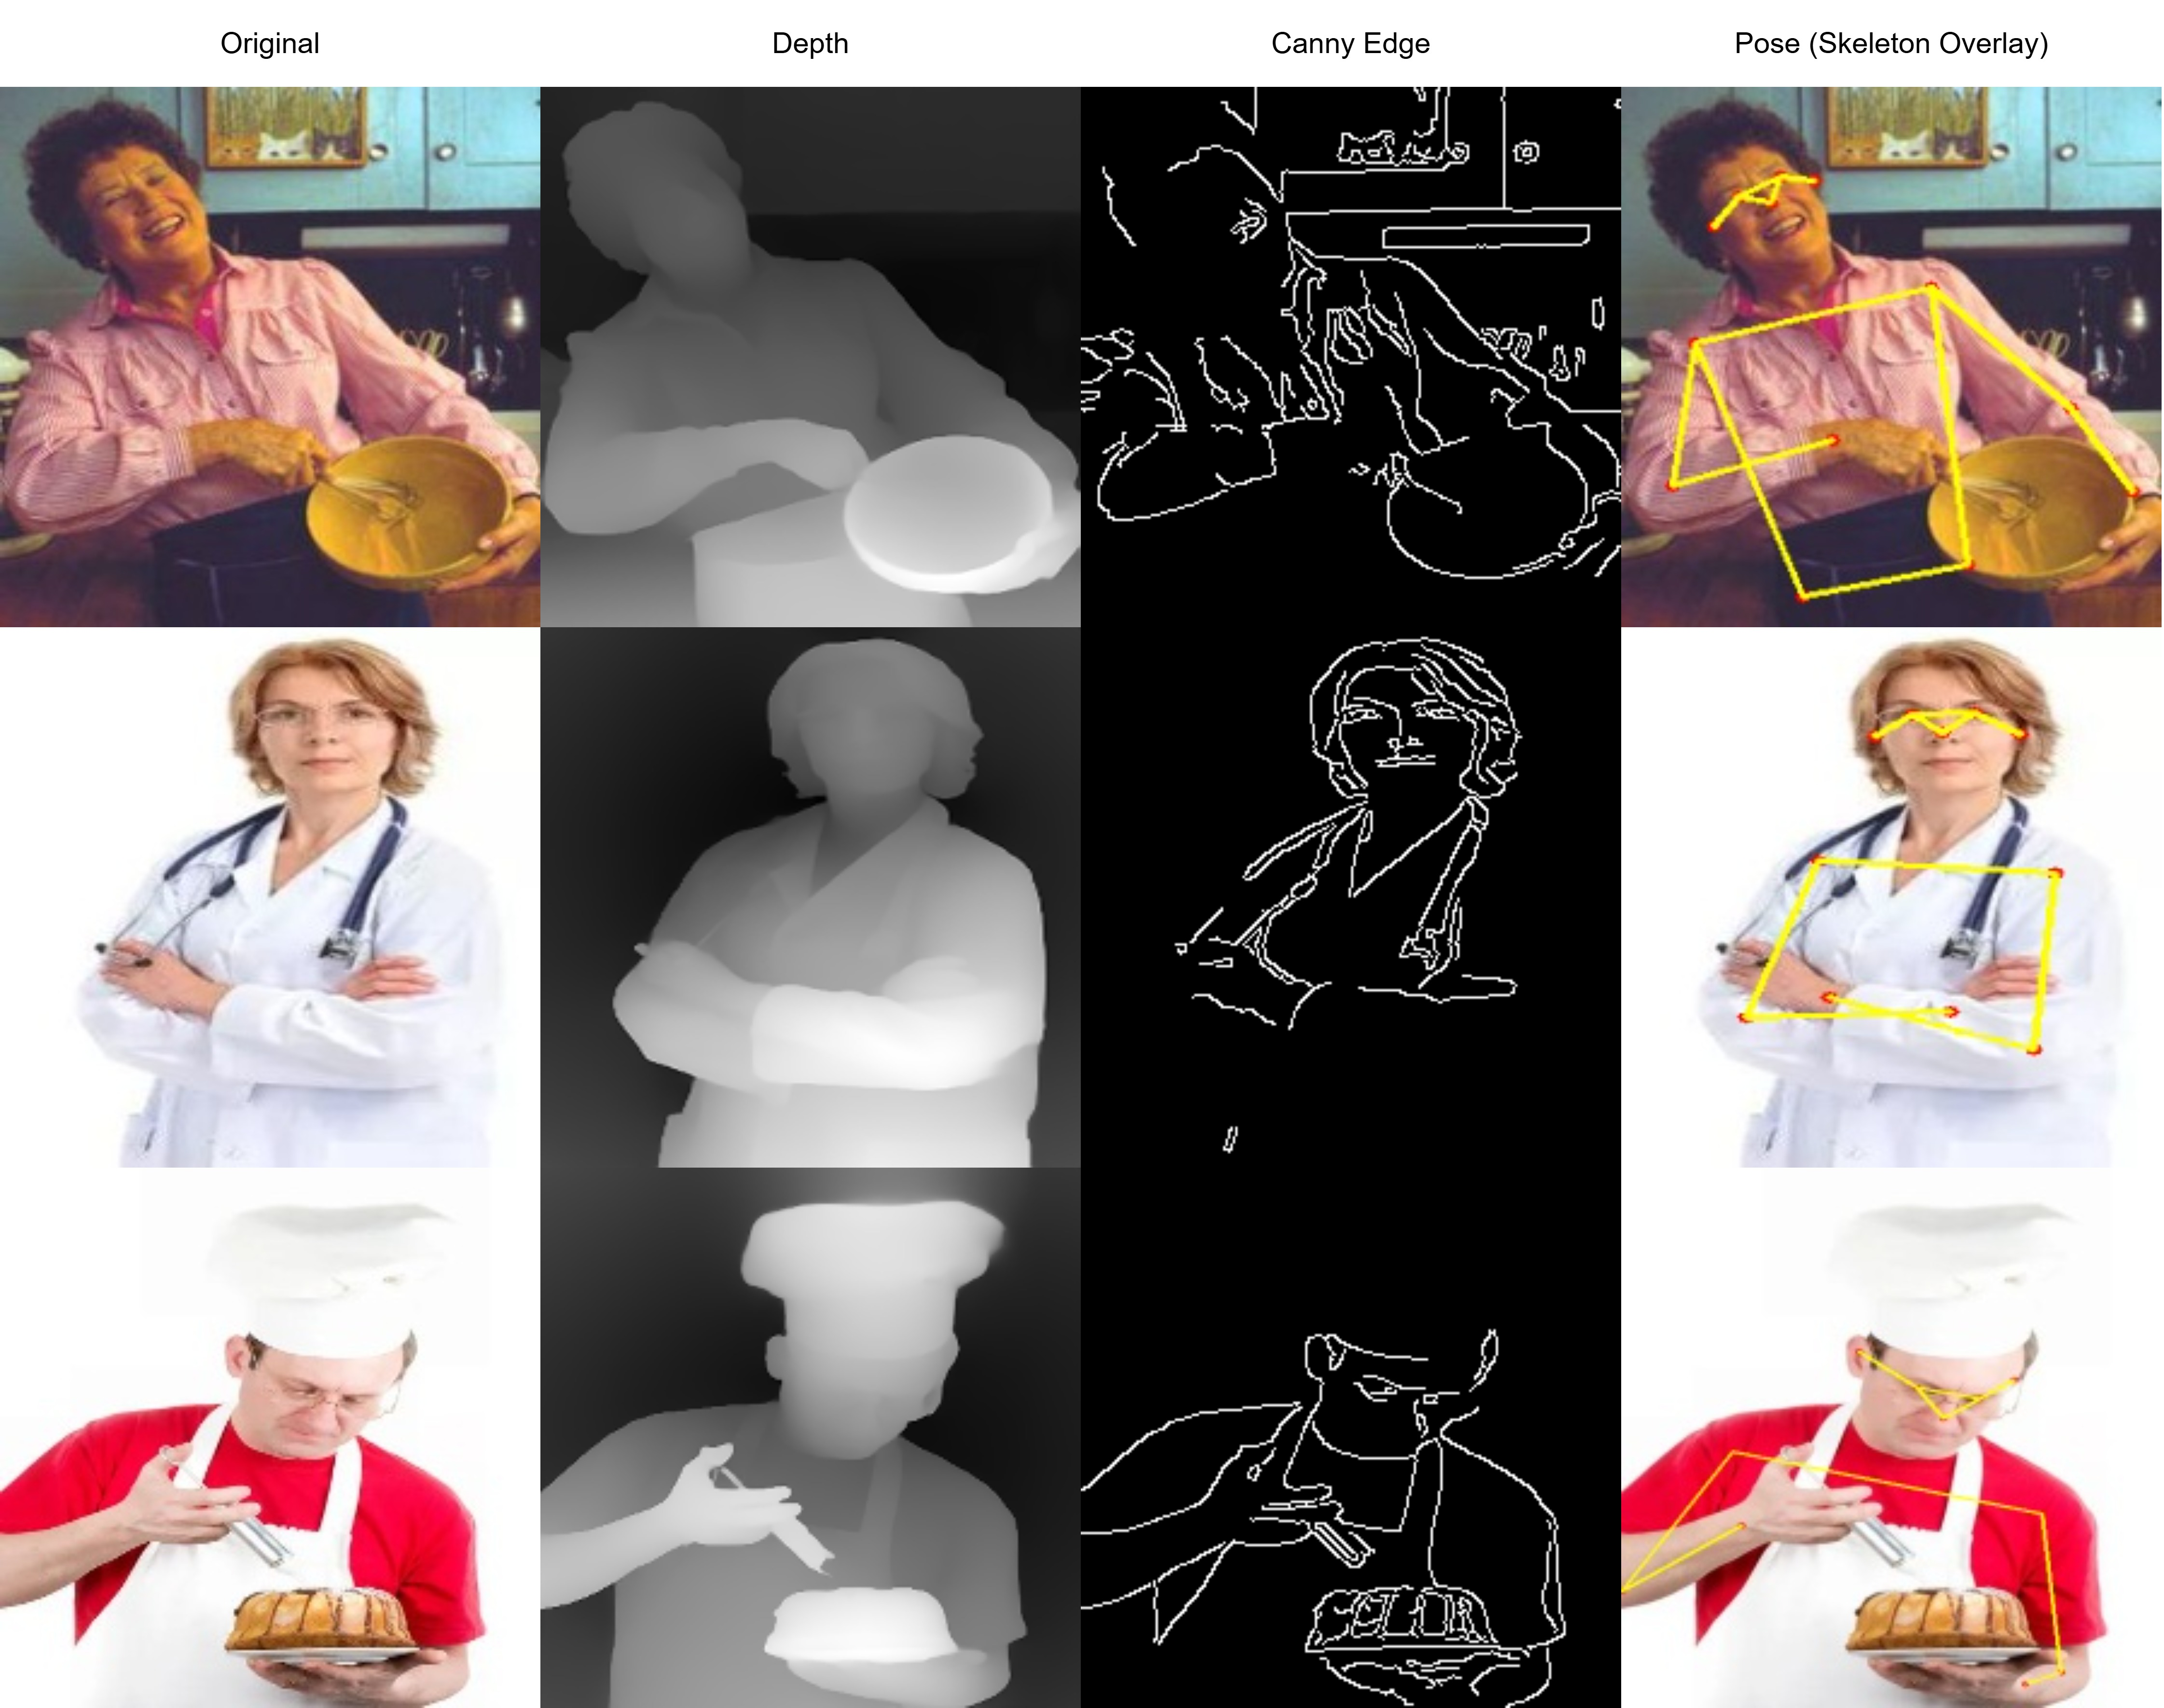
\includegraphics[width=\textwidth, height=0.4\textheight, keepaspectratio]{TD1.jpg}
	\caption{Structural transformations: depth map (Depth-Anything-V2), Canny edge map,
		and YOLOv8l-Pose skeleton overlay. The classifier input for pose is the
		34-dimensional normalised keypoint vector, not the rendered overlay.}
	\label{fig:td_structural_transforms}
\end{figure}

\begin{figure}[H]
	\centering
	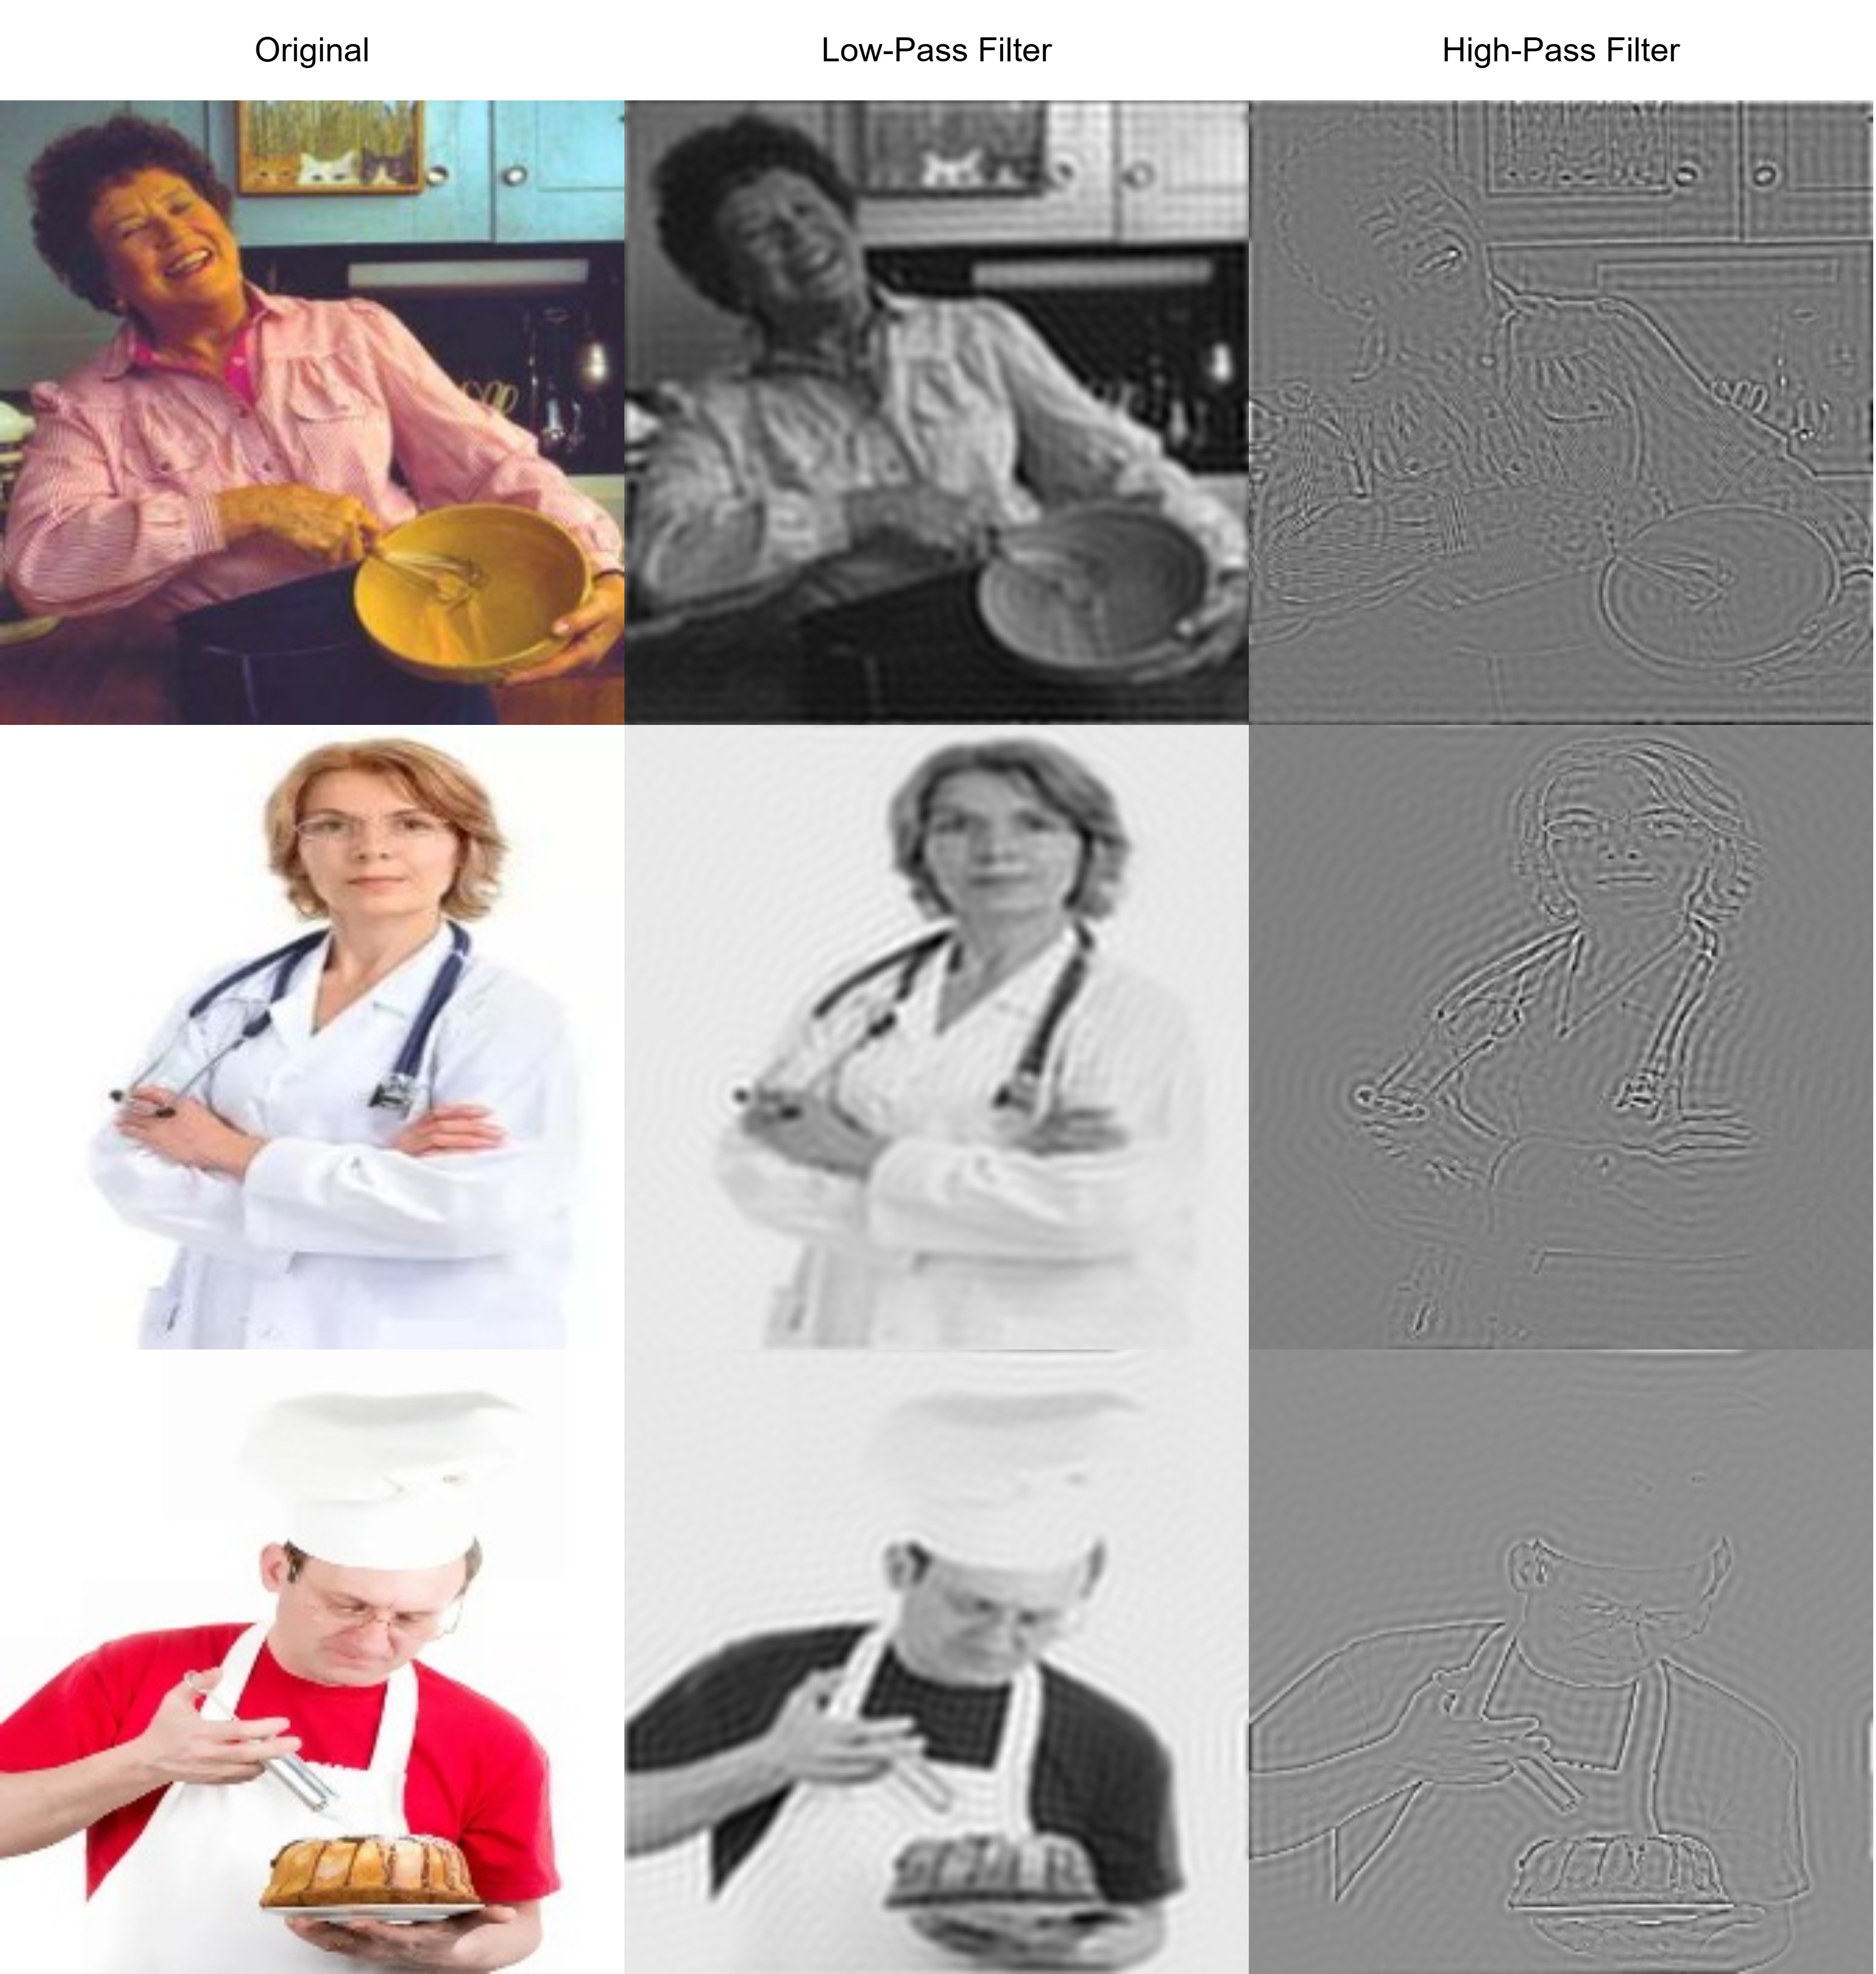
\includegraphics[width=\textwidth, height=0.4\textheight, keepaspectratio]{TD2.jpg}
	\caption{Frequency domain transformations: low-pass reconstruction retaining smooth
		luminance gradients (cutoff $r=40$) and high-pass residual isolating fine
		textures and compression artefacts. Both derived from a single FFT pass per image.}
	\label{fig:td_frequency}
\end{figure}

\begin{figure}[H]
	\centering
	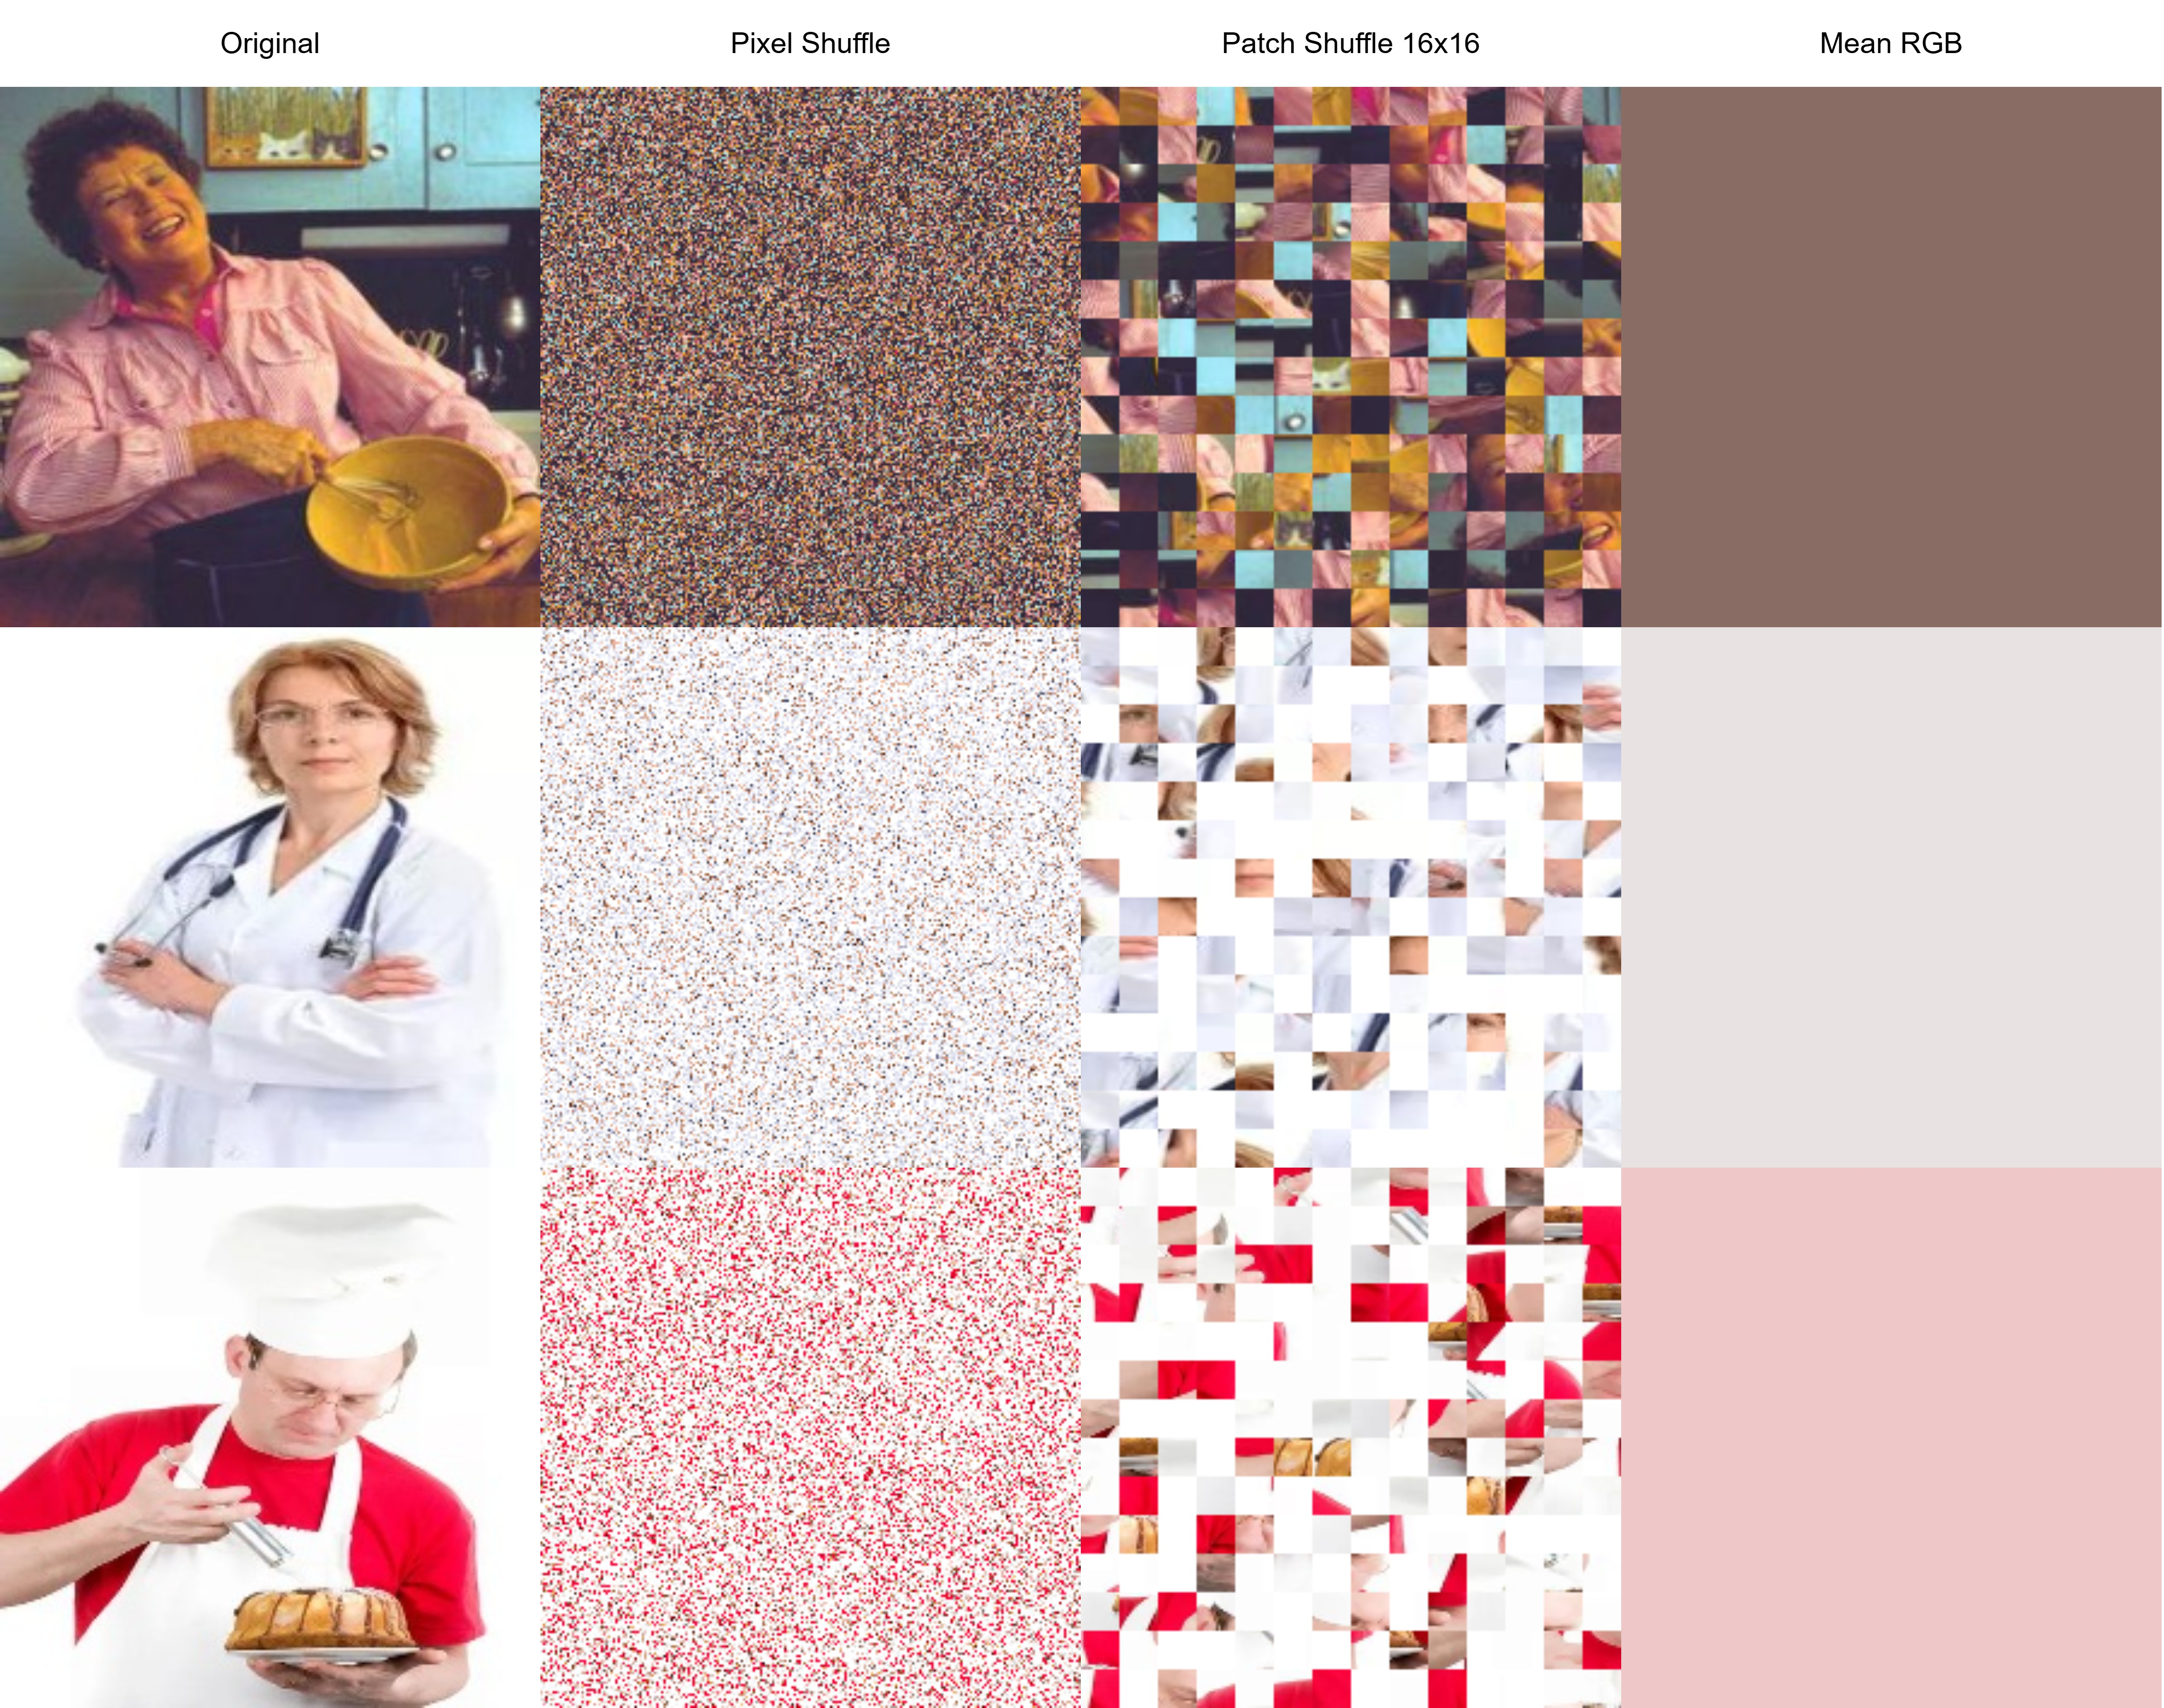
\includegraphics[width=\textwidth, height=0.4\textheight, keepaspectratio]{TD3.jpg}
	\caption{Spatial decomposition: pixel shuffle (global colour preserved, spatial
		structure destroyed), patch shuffle $16\times16$ (local texture preserved,
		global layout disrupted), and mean RGB (uniform per-channel colour fill).}
	\label{fig:td_spatial}
\end{figure}

\begin{figure}[H]
	\centering
	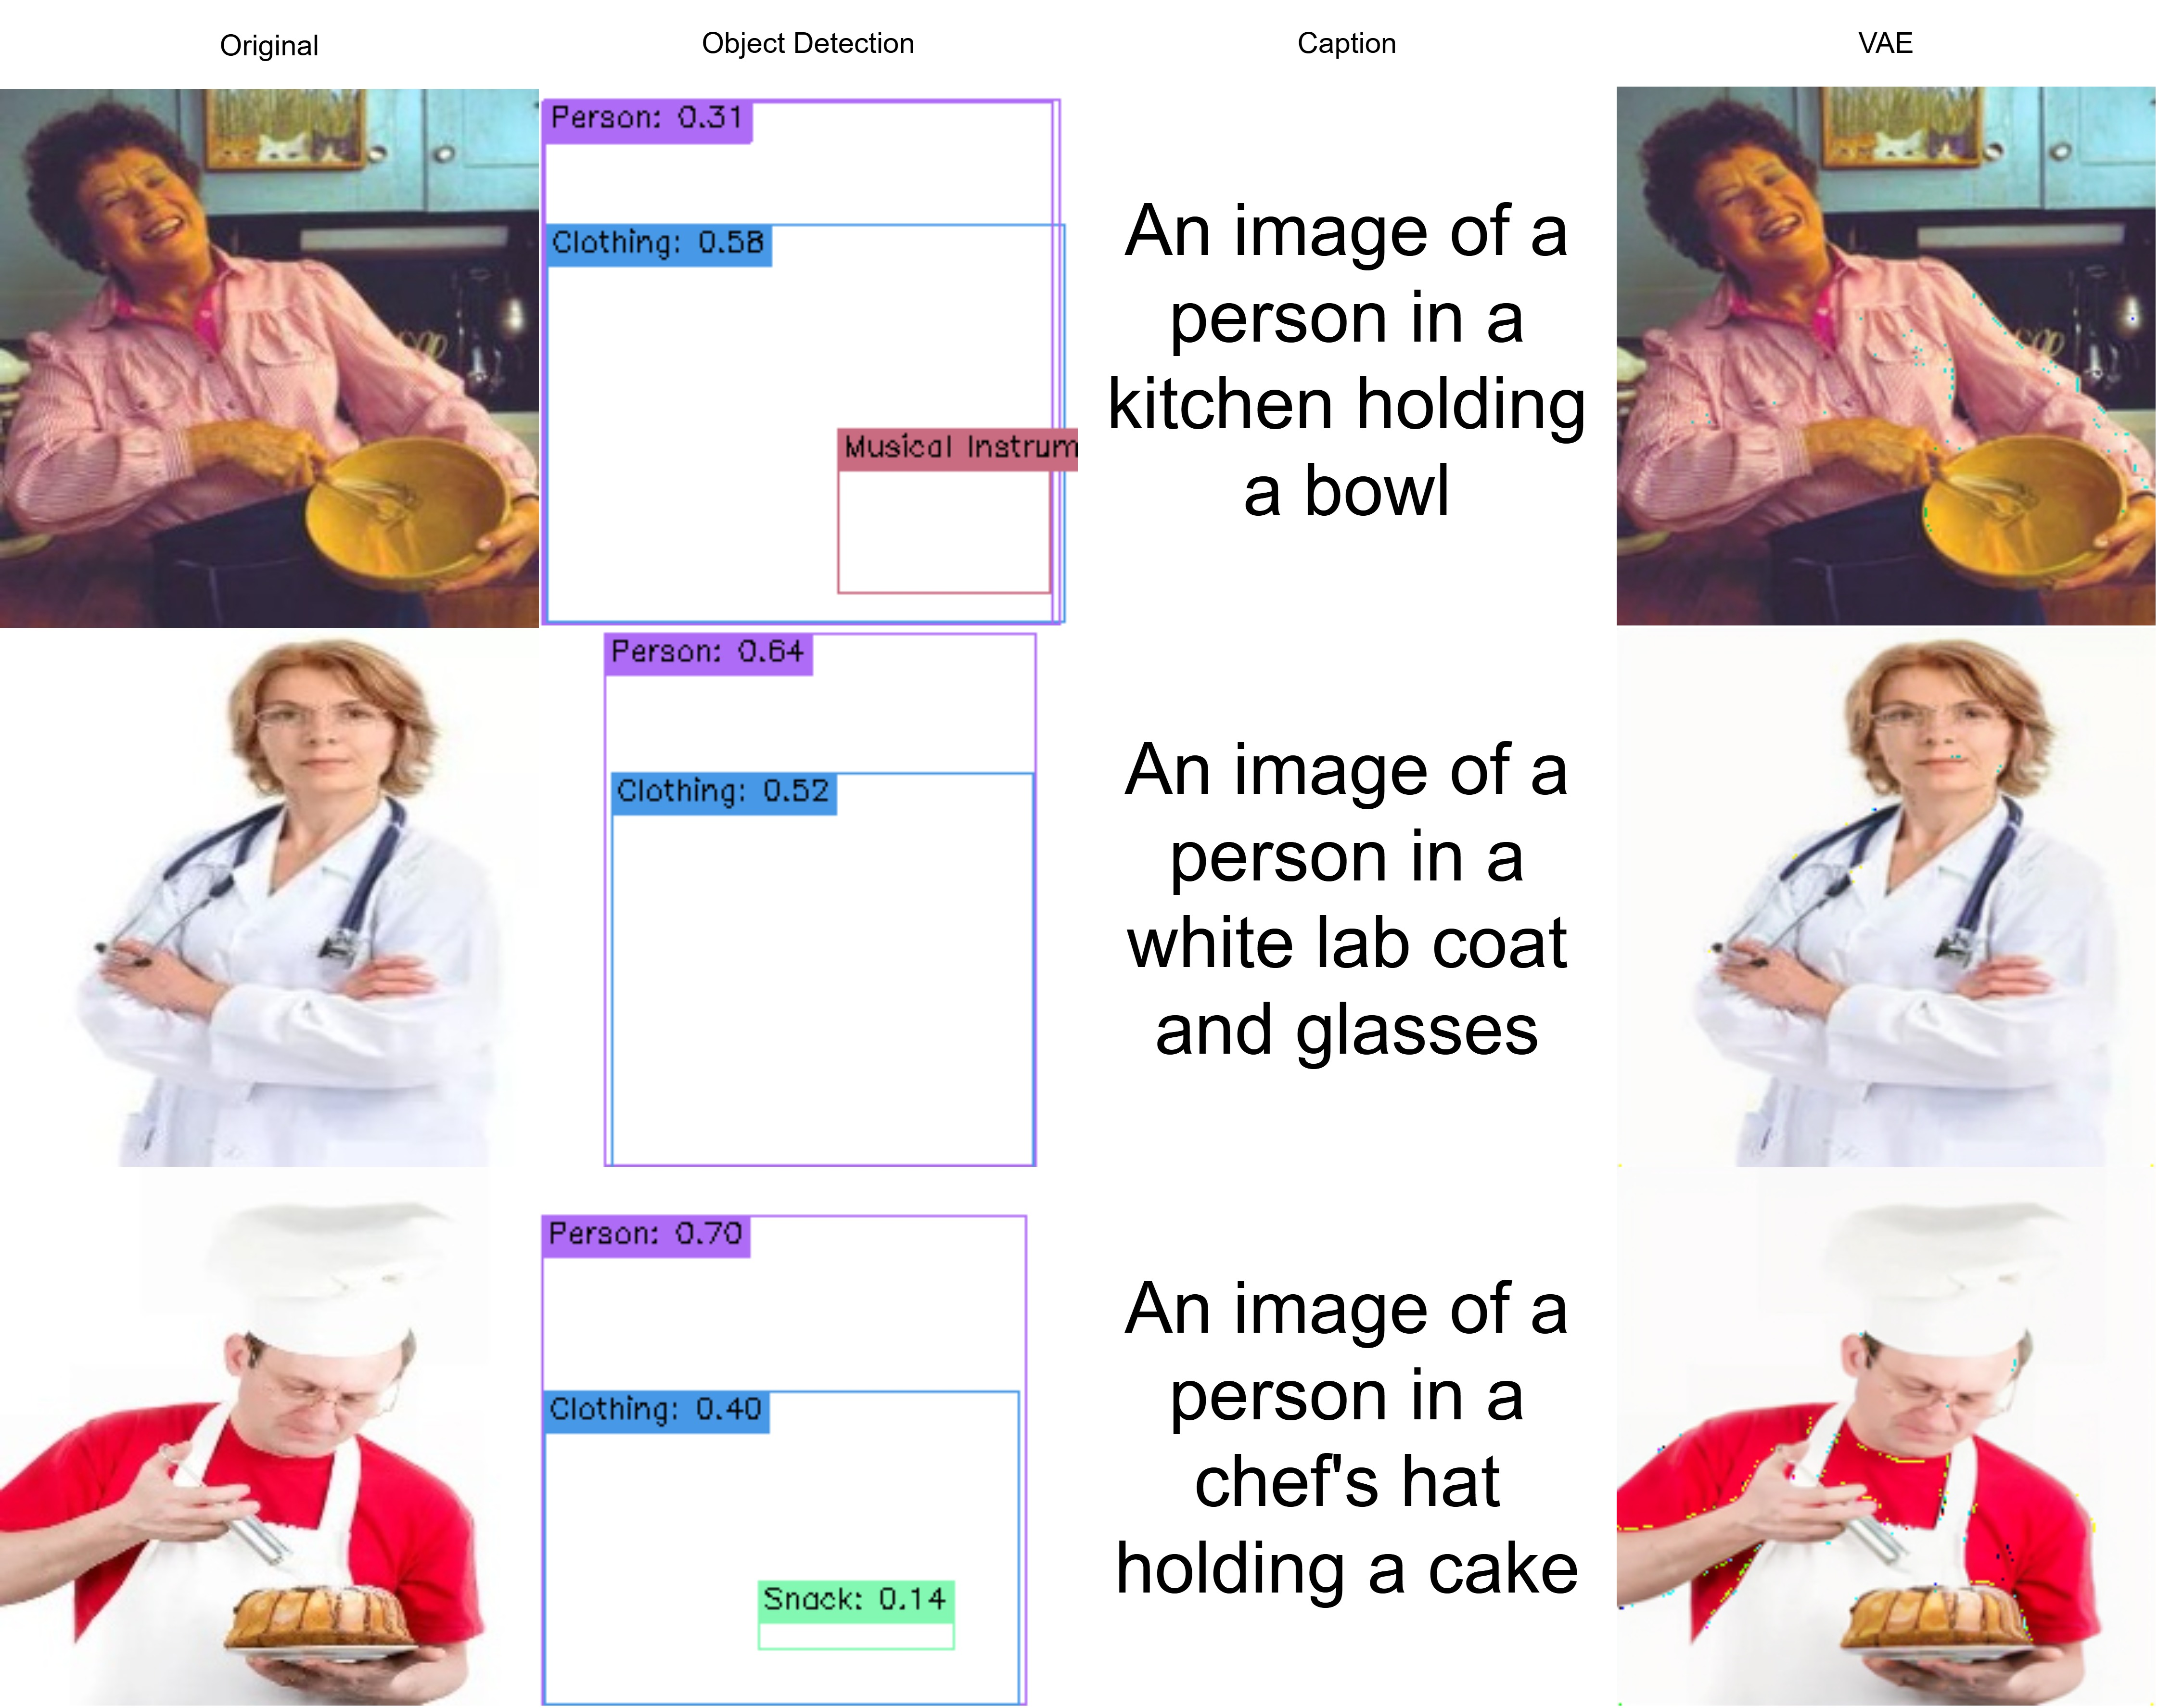
\includegraphics[width=\textwidth, height=0.4\textheight, keepaspectratio]{TD4.jpg}
	\caption{Semantic and latent-space transformations: YOLOv8x object detection
		bounding boxes on white canvas (OpenImages V7), BLIP Large captions with
		gender-neutral remapping, and SD v1.5 VAE reconstructions.}
	\label{fig:td_semantic_latent}
\end{figure}

\begin{figure}[H]
	\centering
	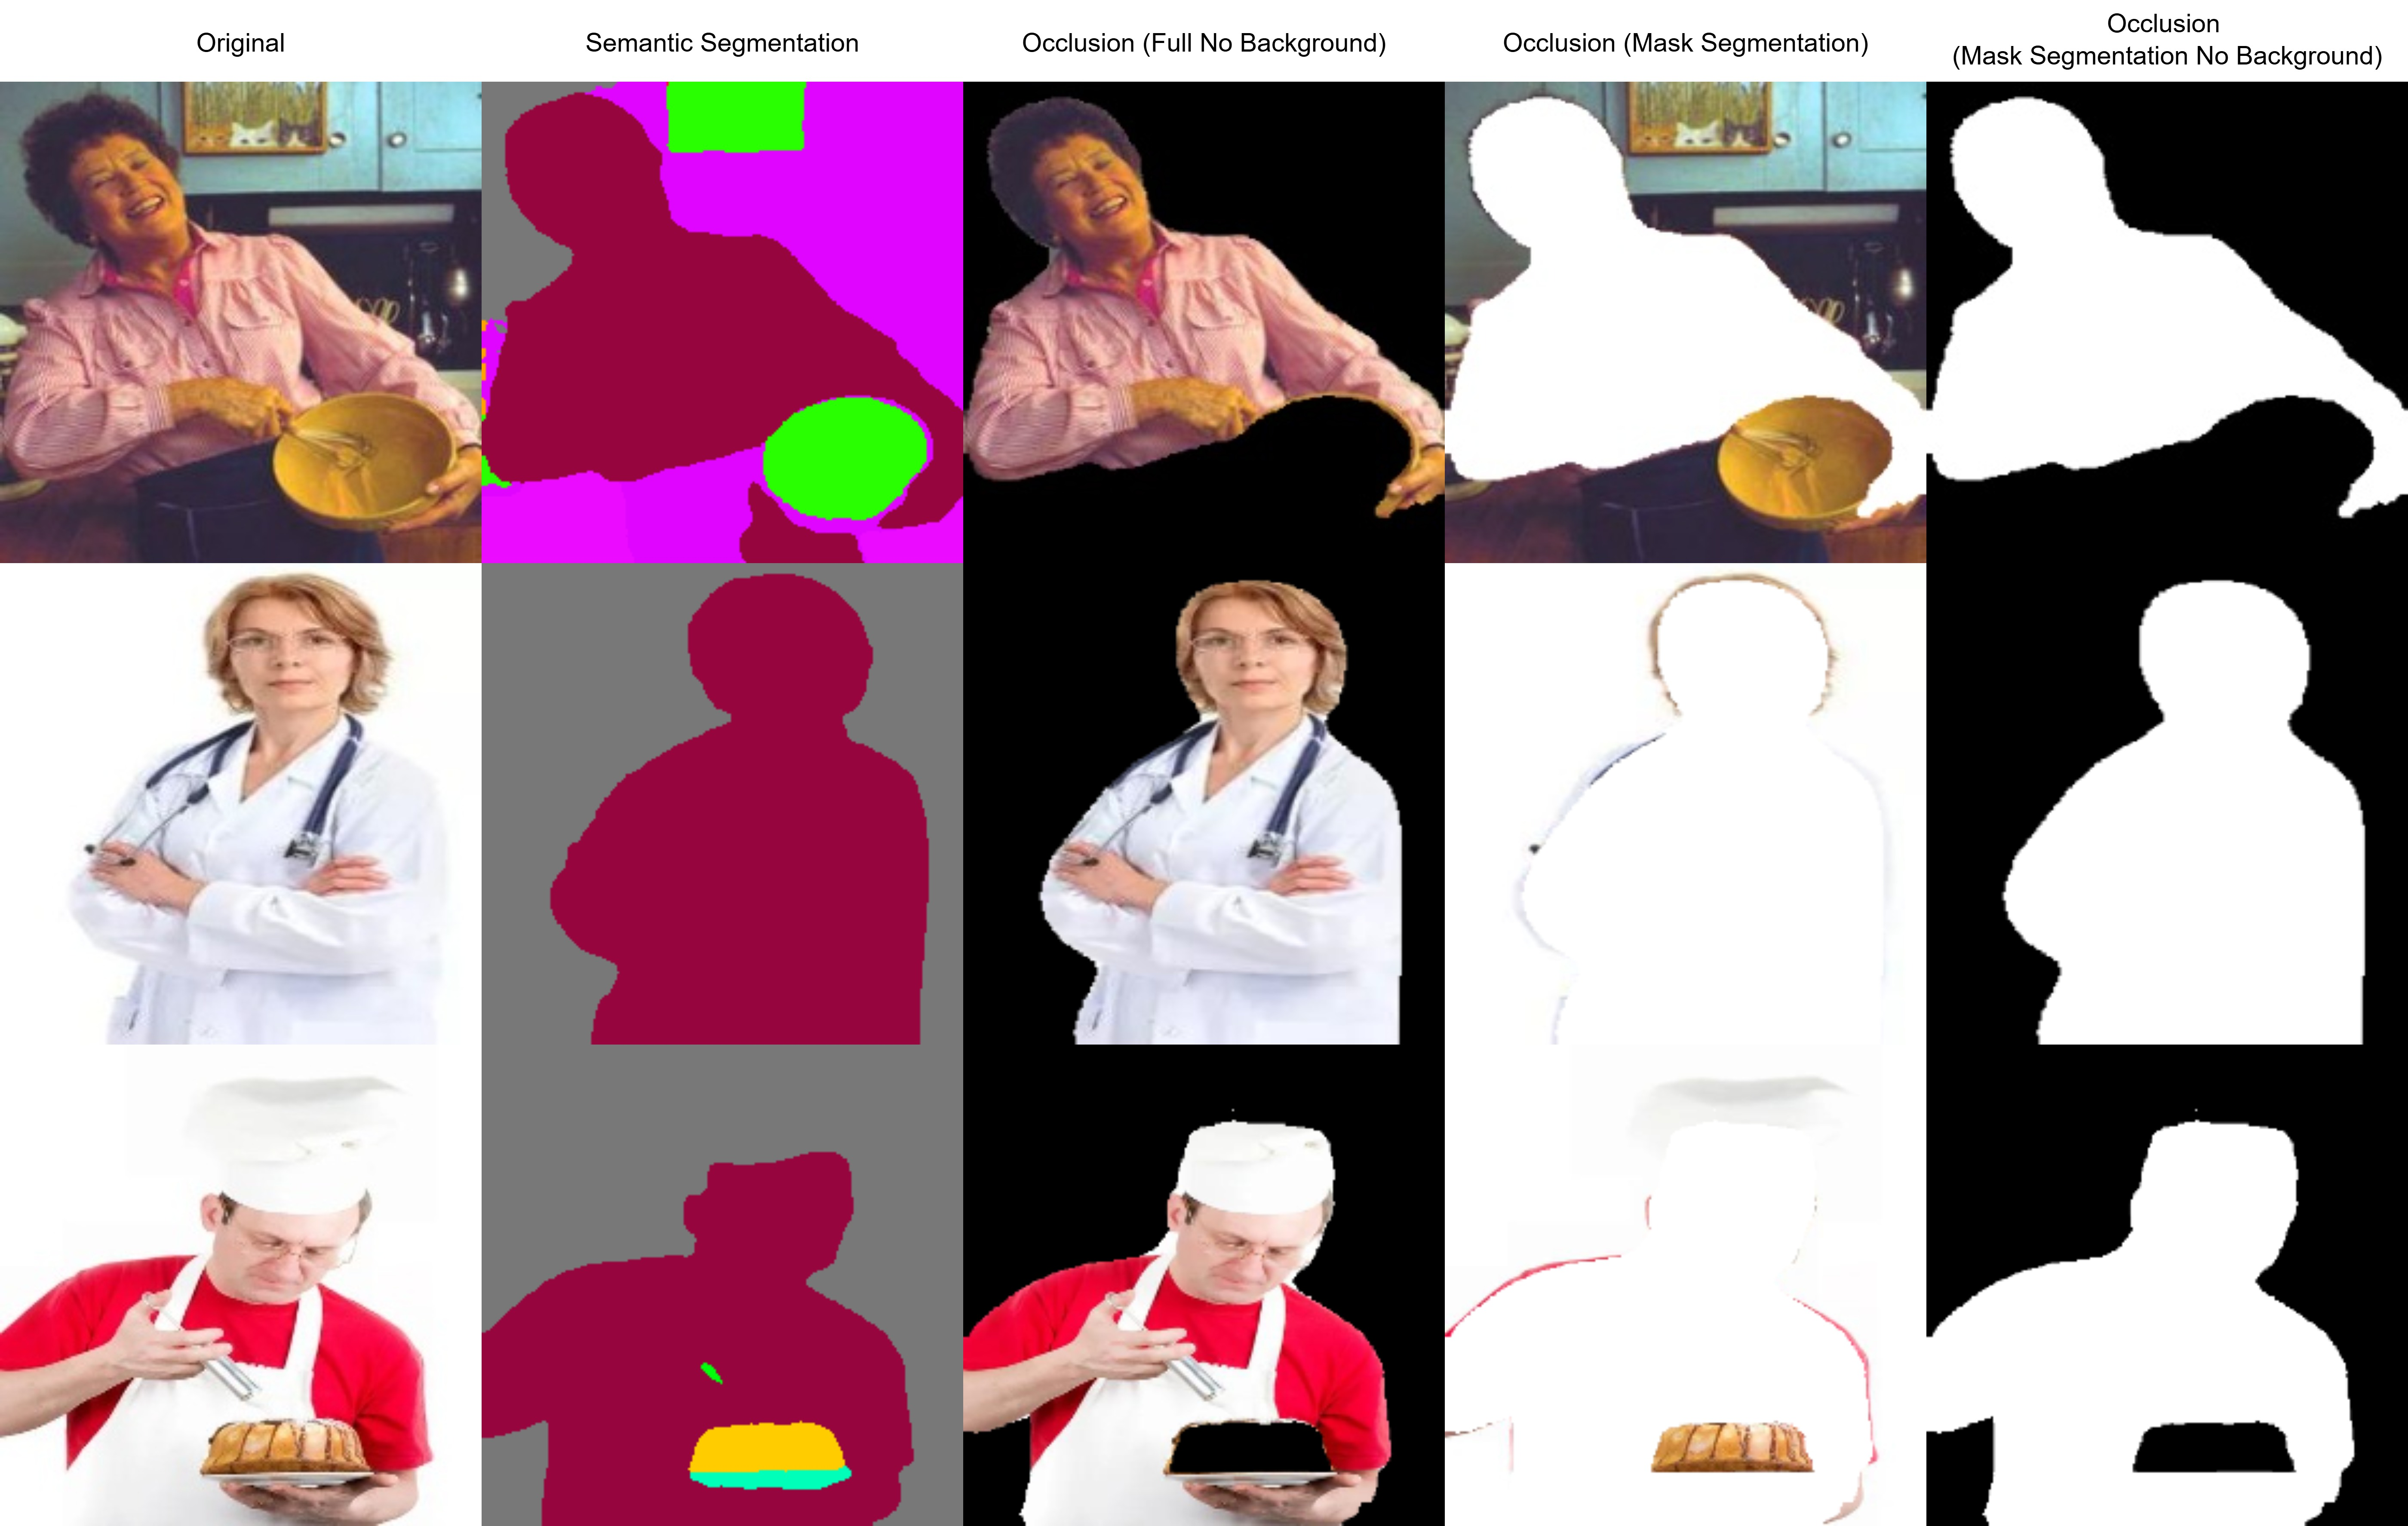
\includegraphics[width=\textwidth, height=0.4\textheight, keepaspectratio]{TD5.jpg}
	\caption{Segmentation and segmentation-derived occlusion: ADE20K pixel-label map
		(Mask2Former), full person isolated (no background), person masked with white
		fill (background retained), and white silhouette on black background.}
	\label{fig:td_segmentation_occlusion}
\end{figure}

\begin{figure}[H]
	\centering
	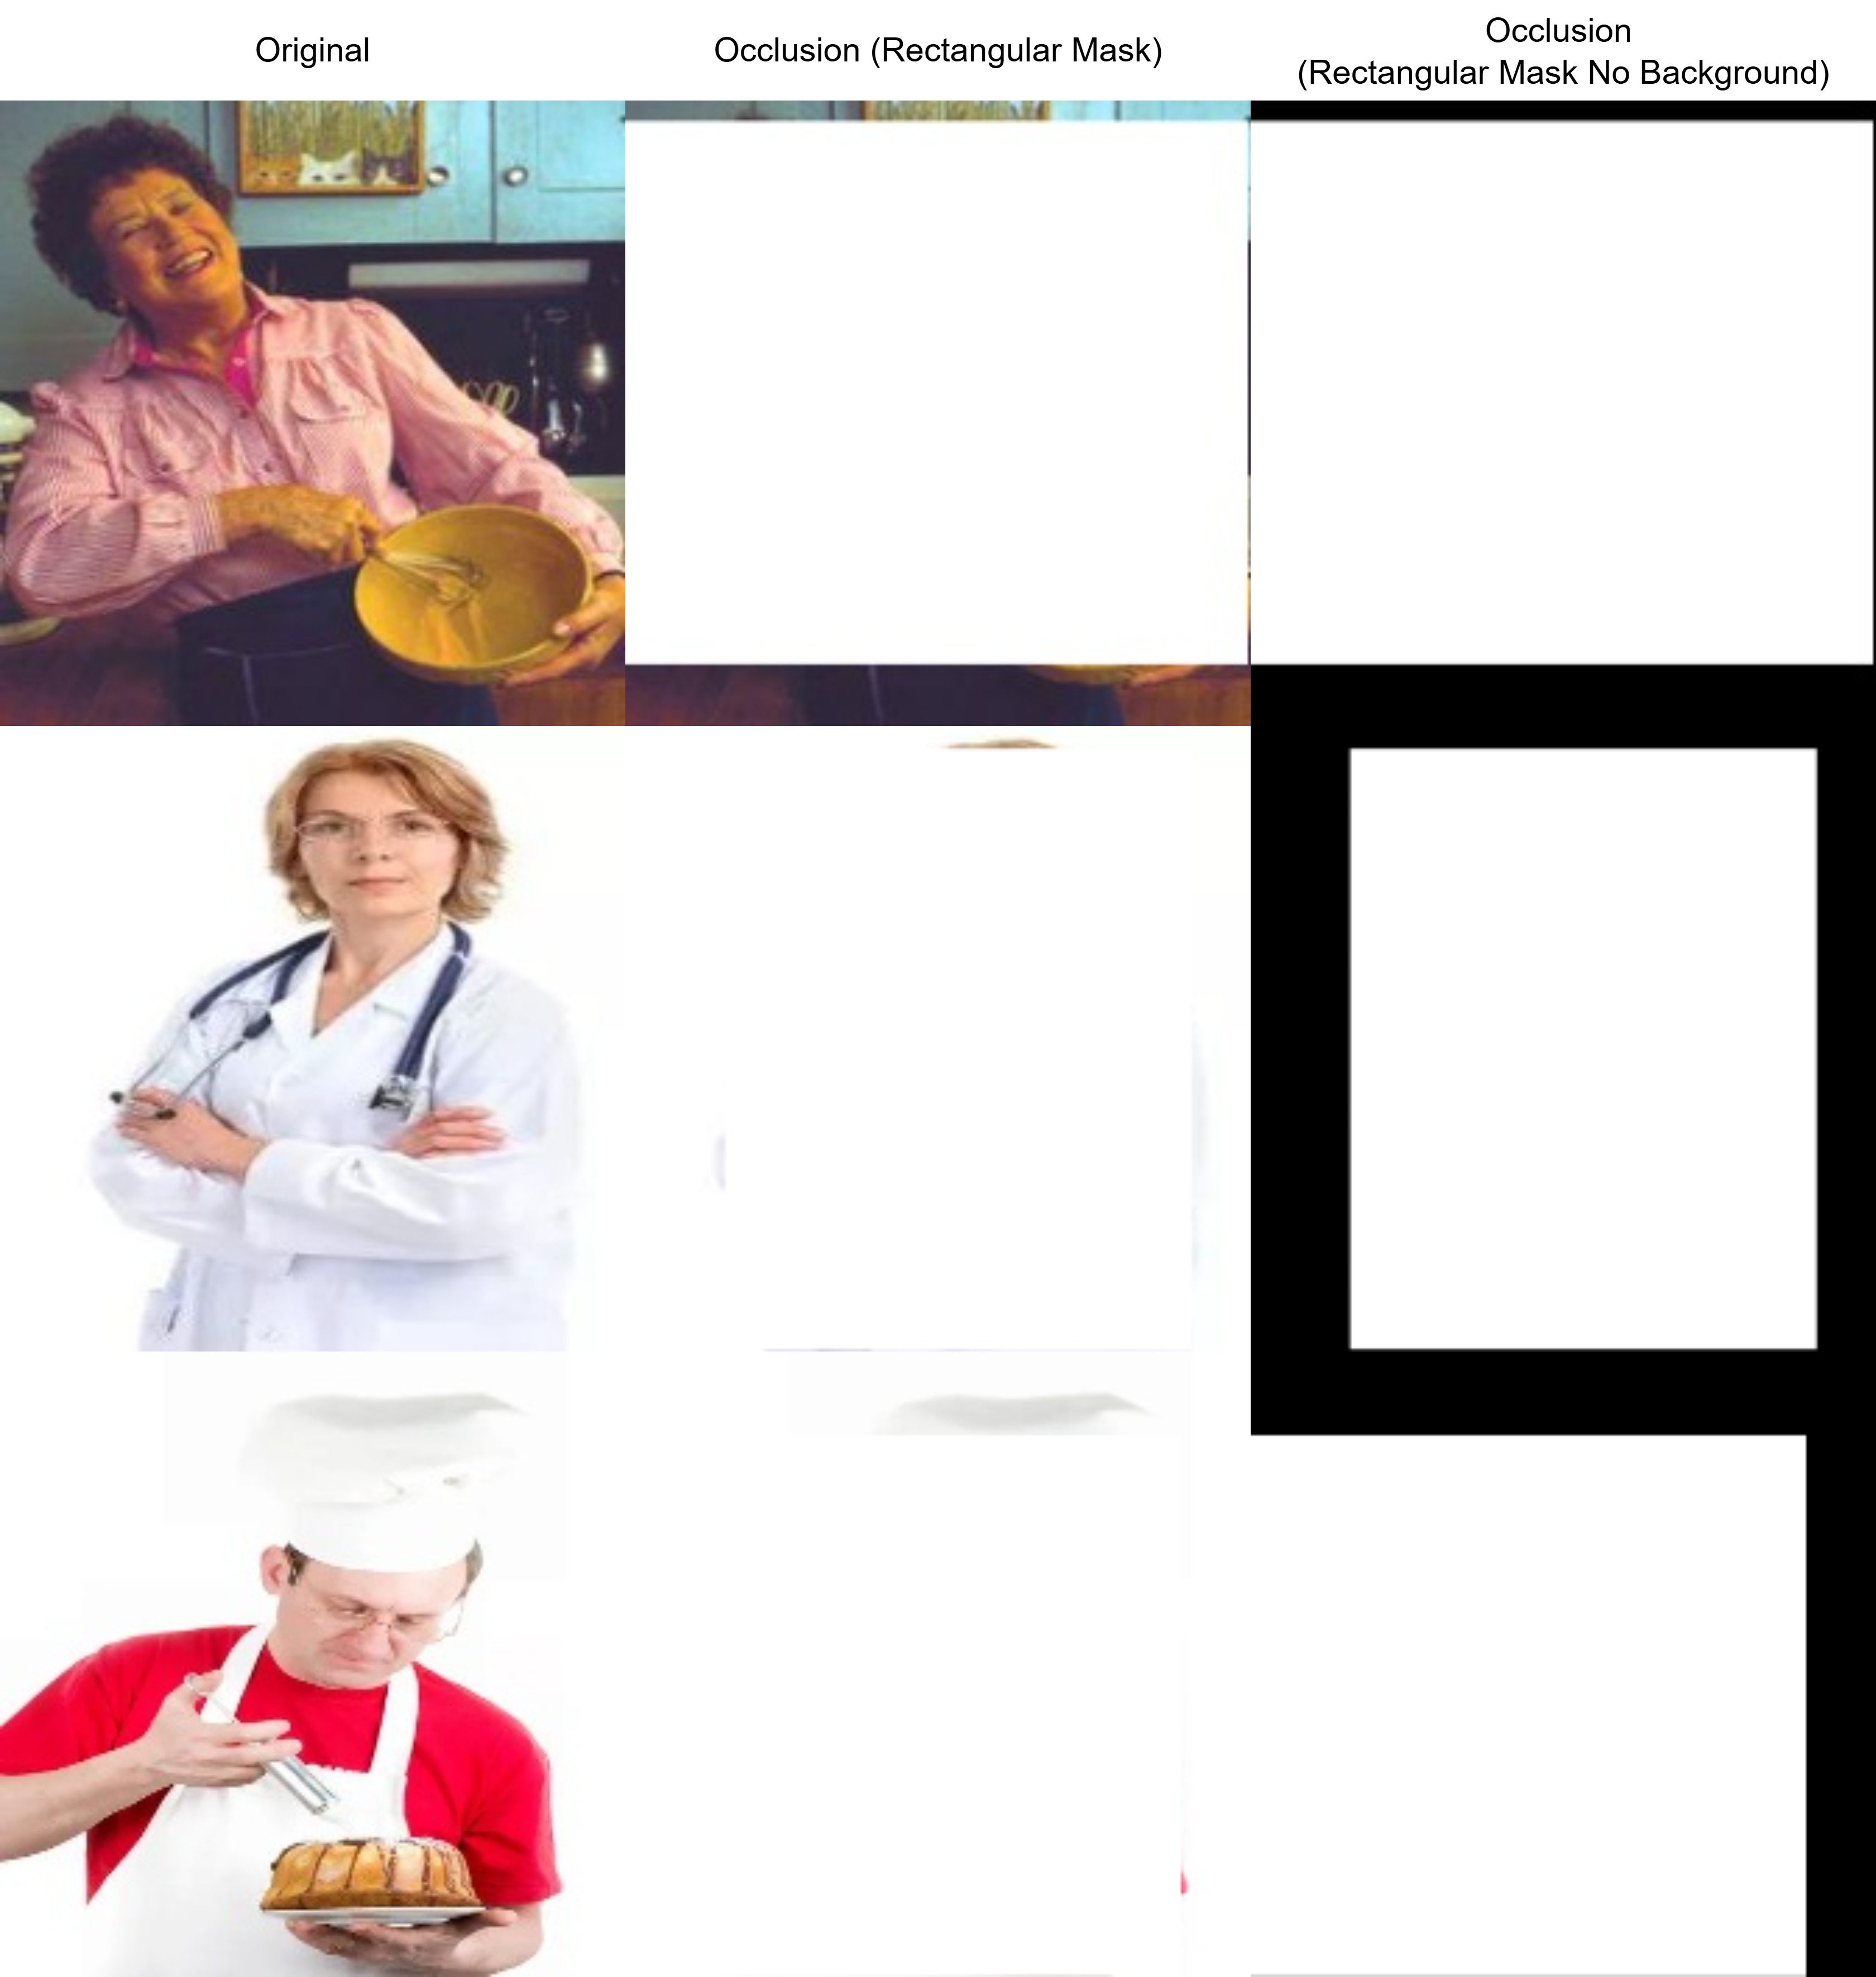
\includegraphics[width=0.75\textwidth, height=0.4\textheight, keepaspectratio]{TD6.jpg}
	\caption{Rectangular occlusion: white rectangle replacing the person region
		(background retained) and inverse mask retaining only the occluded boundary
		region on a black background.}
	\label{fig:td_occlusion_rect}
\end{figure}


\section{Inference-Time Debiasing of Stable Diffusion v1.5}
\label{sec:debiased_generation}

The preceding analyses characterise the spurious features and demographic biases present in Re-LAION-5B and in the standard Stable Diffusion v1.5 generation pipeline. A complementary question is whether inference-time debiasing interventions applied to the same base model can produce measurable shifts in its demographic output distribution. This section describes the debiased generation pipeline used to produce a 10,000-image corpus against which the effectiveness of these interventions is evaluated in Section~\ref{sec:debiasing_evaluation}. Given the computational constraints of this work and the requirement that the base model remain Stable Diffusion v1.5, the analysis is restricted to inference-time approaches; retraining and weight editing methods are acknowledged as potentially more thorough interventions but are outside the scope of the present evaluation.

\subsection{Experimental Design}
\label{subsec:debias_design}

The debiasing experiment was designed as a focused single-profession evaluation rather than a full 200-profession generation run. A total of 10,000 images were generated for the doctor profession, providing sufficient statistical power to detect intervention-driven demographic shifts. Distributing the same generation budget across all 200 professions would yield only 50 images per profession per demographic condition, too few for reliable distributional comparison.

The doctor profession was selected for several converging reasons. First, it exhibits one of the most pronounced demographic skews in the standard Stable Diffusion v1.5 pipeline, making it a demanding test case against which any debiasing effect is clearly measurable. Second, it carries a well-documented real-world demographic baseline, enabling the debiased distribution to be assessed against established reference statistics. Third, computational constraints motivated restricting the debiasing evaluation to a single profession; the doctor prompt was preferred over alternatives because its strong learned prior constitutes a more stringent test of the pipeline's effectiveness. Finally, the doctor prompt has been used as an evaluation case in prior work on occupational bias in text-to-image generation \cite{Bianchi_2023_TTIGenAmplifiesDemographicStereotypes, Luccioni_2023_AnalyzingSocietalRepresentationsDiffusionModels}, supporting direct comparability with the existing literature.

\subsection{Demographic Conditioning}
\label{subsec:debias_itiGEN}

The demographic conditioning component was selected from inference-time approaches capable of steering Stable Diffusion v1.5 without modifying the base model weights, as reviewed in Sections~\ref{subsubsec:iti_gen} and~\ref{subsubsec:fairgen}. FairGen was evaluated but excluded because its adapter-based latent direction discovery did not produce sufficiently coherent Stable Diffusion v1.5 outputs for reliable large-scale evaluation. ITI-GEN was adopted instead because it produced coherent outputs while achieving the required demographic conditioning.

ITI-GEN \cite{Zhang_2023_ITIGEN} learns a set of inclusive token embeddings that steer the diffusion model toward a more balanced demographic distribution without modifying model weights. Token embeddings were trained on CCv2 \cite{Porgali_2023_CCv2} across two attribute axes: gender, represented by female and male categories, and skin tone, spanning the ten-point MST scale. This produced learned perturbation embeddings indexed over all gender--skin tone combinations. The training prompt was \texttt{"an image of a person"}, following ITI-GEN's neutral prompt convention. The trained embeddings were applied to the generation prompt \texttt{"A picture of a doctor"} via the \texttt{prompt\_prepend} mechanism, concatenating inclusive embeddings with the CLIP text encoding before passing the combined representation to the UNet cross-attention layers.

\subsection{Pose Conditioning via ControlNet}
\label{subsec:debias_controlnet}

A fixed canonical pose was enforced across all debiased images using ControlNet \cite{LZhang_2023_ControlNet} with OpenPose conditioning. The conditioning image was a single reference pose skeleton depicting a neutral standing figure, applied at a ControlNet scale of 0.6. Without a fixed structural constraint, the model's learned pose prior may itself be demographically skewed, allowing body-geometry variation to confound demographic annotation. A canonical pose therefore reduces pose-correlated compositional confounds in the debiased corpus.

\subsection{Colour Alignment}
\label{subsec:colour_alignment}

ITI-GEN operates through semantic text conditioning and does not directly constrain image colour distributions. A complementary inference-time colour alignment strategy was therefore added to steer the denoising trajectory toward a neutral reference colour distribution derived from the standard SD v1.5 doctor generation corpus. Two colour-guidance approaches reviewed in Section~\ref{subsubsec:colour_guidance} were implemented and compared: SW-Guidance and Chamfer colour alignment.

SW-Guidance \cite{Lobashev_2025_SWGuidance} applies Sliced Wasserstein Distance guidance at each denoising step by decoding the current latent to pixel space and computing a gradient signal that minimises the SWD between the decoded image's colour distribution and that of a reference. Despite producing favourable preliminary colour distributions, SW-Guidance was excluded on throughput grounds: the repeated decode--gradient--encode operations at each denoising step result in inference times incompatible with generating 10,000 images within the available computational window.

The Chamfer colour alignment approach of Shum et al.\ \cite{Shum_2025_ColorAlignment} performs colour steering directly in latent space without decoding at each step. A reference image is blurred and encoded to a latent representation at the start of generation. At each DDPM backward step, the predicted clean sample $\hat{x}_0$ is projected toward the reference latent distribution using an iterative Chamfer distance matching procedure: nearest-neighbour correspondences between spatial positions of the current and reference latents are established, a displacement field is computed from matched correspondences, and the projected latent is blended back into the denoising step via a learning-rate-scaled update. Because the Chamfer projection operates entirely in latent space, it avoids per-step decode--encode overhead and achieves throughput comparable to standard generation. Chamfer colour alignment was therefore selected for the full-scale debiased run.

\subsection{Generation Configuration}
\label{subsec:debias_config}

The debiased corpus was generated using Stable Diffusion v1.5 (\texttt{runwayml/stable-diffusion-v1-5}) with a fine-tuned VAE (\texttt{stabilityai/sd-vae-ft-mse}), producing $512 \times 512$ pixel images. The generation prompt was \texttt{"A picture of a doctor"}, with classifier-free guidance at a scale of 7.0. Unlike the standard generation pipeline, which used $s = 1.0$ to minimise inference-time amplification of learned priors, the debiased pipeline uses the standard deployment scale to ensure that the model's demographic priors are fully active. This provides a more demanding test of whether the debiasing interventions can override those priors. The denoising schedule used 50 inference steps over the canonical 1{,}000-step scaled-linear noise schedule, with $\beta_{\text{start}} = 0.00085$ and $\beta_{\text{end}} = 0.0120$, following the standard Stable Diffusion v1.5 configuration. A fixed negative prompt was applied throughout: \texttt{"longbody, lowres, bad anatomy, bad hands, missing fingers, extra digit, fewer digits, cropped, worst quality, low quality"}.

The full generation space comprised twenty demographic combinations: two gender categories, female and male, crossed with ten skin tone levels, MST~1--10, from the CCv2 attribute set. Five hundred images were generated per combination, yielding a total corpus of 10{,}000 images. A base random seed of 42 was used, with per-image seeds derived deterministically as $\text{seed} + n$ for iteration index $n$, ensuring full reproducibility across all combinations.

ITI-GEN inclusive token embeddings trained on CCv2 \cite{Porgali_2023_CCv2} under the training prompt \texttt{"an image of a person"} were used to condition the generation prompt via the \texttt{prompt\_prepend} mechanism, as described in Section~\ref{subsec:debias_itiGEN}. ControlNet OpenPose conditioning (\texttt{lllyasviel/control\_v11p\_sd15\_openpose}) was applied at a conditioning scale of 0.6 using a single fixed reference pose skeleton (\texttt{basic\_pose.jpg}), enforcing a canonical standing posture across all generated images as described in Section~\ref{subsec:debias_controlnet}. LCM-LoRA was not used because its reduced step count, combined with per-step Chamfer projection, produced images insufficiently coherent for annotation and probing.

The Chamfer colour alignment projection was applied to the predicted clean sample $\hat{x}_0$ at every denoising step where the DDPM timestep $t > 600$, corresponding to approximately the first twenty of the fifty inference steps. Restricting projection to early high-noise timesteps follows the placement strategy of Shum et al.\ \cite{Shum_2025_ColorAlignment}, where colour steering applied at low-noise timesteps risks corrupting fine-grained semantic detail. The projection used a learning rate of 0.05 and a blur factor of 5. The blur operation downsamples the reference image to one-fifth of its spatial resolution before re-upsampling prior to VAE encoding, suppressing high-frequency texture in the reference signal and retaining only the broad colour distribution. The colour reference image was a uniform-fill image derived from the mean RGB of the standard SD v1.5 doctor generation corpus, providing a neutral colour prior without encoding any scene-level content.